% Author - Jon Arnt Kårstad, NTNU IMT
\documentclass{report}

% Importing document settings from our file "packages.sty"
\usepackage{setup}

% Beginning of document
\begin{document}
\import{./Sections/}{FrontPage}
% Inserting title page


% Defining front matter settings (Norsk: innstillinger for forord m.m.)
\frontmatter
\newpage
\thispagestyle{empty}
\mbox{}
\chapter*{Abstract}
{\setstretch{1.35} % Adjust line spacing
\begin{tabbing}
\setstretch{1.5} % Adjust line spacing
\hspace{2cm}\=\hspace{1.5cm}\=\kill % set the tab stops
Title: \> \>Securing the Software Development Life Cycle \\
Date: \> \> 22.05.2023 \\ 
\\
Participants: \> \> Anniken Arildset \\ \> \> Celina Brynildsen \\ \> \> Sebastian Hestsveen \\ \> \> Thea Urne \\
\\
Supervisor: \> \> Filip Holik, Visiting Researcher/Research Assistant, \\\> \> Department of Information Security and Communication Technology \\
\\
Employer: \> \>  Astri Marie Ravnaas, Norges Bank Investment Management (NBIM) \\
\\
Keywords: \> \> AWS, DevSecOps, GitHub, Information Security, Infrastructure as Code,\\\> \> SDLC \\
\\
Pages: \> \> Xx \\
Attachments: \> \> Xx \\
Availability: \> \> Open \\
\\
Abstract: \> \> Many security measures can be integrated into the process as soon as\\ \> \> the  code is uploaded to GitHub, and there are multiple scans that can\\ \> \> be performed during the transition from GitHub to the cloud\\ \> \> environment to ensure that the security is maximized before deploying\\ \> \>  the application to the cloud. The group has built an automated pipeline \\ \> \>and added tools.
\end{tabbing}
}

\newpage
\chapter*{Sammendrag}

\begin{tabbing}
\hspace{2cm}\=\hspace{3cm}\=\kill % set the tab stops

Tittel: \> \> Securing the Software Development Life Cycle \\
Dato: \> \> 22.05.2023 \\ 
\\
Deltakere: \> \> Anniken Arildset \\ \> \> Celina Brynildsen \\ \> \> Sebastian Hestsveen \\ \> \> Thea Urne \\
\\
Veileder: \> \> Filip Holik, Forsker/Vitenskapelig assistent, \\\> \> Institutt for informasjonssikkerhet og kommunikasjonsteknologi \\
\\
Oppdragsgiver: \> \>  Astri Marie Ravnaas, Norges Bank Investment Management (NBIM) \\
\\
Nøkkelord: \> \> Informasjonssikkerhet, SDLC, DevSecOps, AWS, GitHub \\
\\
Antall sider: \> \> Xx \\
Antall vedlegg: \> \> Xx \\
Tilgjenlighet: \> \> Åpen \\
\\
Sammendrag: \> \>Mange sikkerhetstiltak kan integreres i prosessen så snart kode lastes \\\> \>opp til GitHub, og det er flere scanninger som kan være utført under \\\> \>overgangen fra GitHub til skymiljøet for å sikre at sikkerheten er \\\> \>maksimert før man distribuerer applikasjonen til skyen. Gruppen har \\\> \>bygget en automatisert pipeline og lagt til verktøy og tiltak som anses\\\> \> som beste praksis i bransjen. Verktøyene ble valgt basert på\\\> \> brukervennlighet og tidligere dokumentasjon av lignende testing.

\end{tabbing}



\tableofcontents

\listoffigures
\listoftables
%\lstlistoflistings

\printglossary[type=\acronymtype]
\printglossary
\newpage


\mainmatter

% Defining main matter settings (Norsk: innstillinger for hoveddelen av teksten)

% Introduction explaining this LaTeX-template
\newpage
\thispagestyle{empty}
\mbox{}
\chapter{Introduction}

\section{Background} %Hvorfor vi fikk oppgaven 
\acrlong{nbim}, from now on referred to as \acrshort{nbim}, is a division within the central bank responsible for overseeing the Government Pension Fund of Norway, which has a worth of 14,000 billion Norwegian kroner \cite{nbimwebsite}. Due to its significant value, the fund is a major target for potential malicious actors. It faces an average of three severe cyber attacks daily, totalling around 100,000 attacks each year. Out of these, more than 1,000 are considered significant threats \cite{nbimattacks}. Therefore, it is crucial for \acrshort{nbim}, as well as other organizations, to ensure the security of their systems and applications before deploying them into their cloud services. 
\\~\\
\acrlong{sdlc} (\acrshort{sdlc}) describes how software applications are built - from planning through implementation and running in production. It also includes ensuring security at the different stages of software development. In order to accommodate frequent deployments to production, it is essential to automate the security testing by building it into the deployment pipeline. Security testing can further benefit from shift-left, where testing is done as early as possible in the pipeline. Implementing a strong and secure software development life cycle is essential to prevent attacks from hackers and other malicious actors on the application. Securing the \acrshort{sdlc} is a large and actively developed area with much industry interest. Demonstrating the integration and practical application of various tools and methods can benefit both \acrshort{nbim} and other organizations.

\subsection{Problem area}
The technology industry is in constant development. With this development comes a rapidly expanding threat landscape. How developers approach IT and security must accompany this rapid development to secure systems and applications from malicious actors. Securing the \acrlong{sdlc} has become a common topic in the tech industry, and many resources are available to help organizations implement best practices and adequate security measures. However, finding the appropriate resources can take time, and automating the complete distribution process and automated testing using multiple tools can be time-consuming. Therefore, NBIM is looking for proof of concepts for building a secure pipeline using best practices and implementing multiple security tools to scan for security misconfigurations and vulnerabilities at crucial pipeline stages. 

 
\section{Scope limitations}
The thesis covers all phases of the \acrlong{sdlc}, and gives an overview of each phase and the importance of securing them. The phases consist of planning, implementation, testing, deployment, and maintenance. However, due to the scope, only the last four phases will be the main priority for testing purposes and building a secure pipeline from GitHub to \acrshort{aws}. The group has also decided not to focus on \gls{shift-left} testing within the life cycle, as the focus is on the later phases. 
\\~\\
As a part of the thesis, the group utilized \acrshort{aws} as it was required to use. However, considering the vastness of the \acrshort{aws} platform, the group chose not to explore the tools available within \acrshort{aws} extensively. Instead, the group opted to use the tools necessary at that time and were relatively simple to implement rather than focusing too much on the tools one could use to build the pipeline.
\newpage
\section{Target group}
The thesis has multiple target groups. The primary target group is \acrshort{nbim}, the stakeholder for this thesis, for whom the group will produce a comprehensive report on the task assigned to them. However, this report has the potential to benefit other organizations, and therefore, another target group is any organization that utilizes the \acrshort{sdlc} and aims to improve its security.

\section{Goals}
\subsection{Performance goals}
\begin{itemize}
    \item[-] P1: Collaborate effectively with team members to ensure the timely completion of tasks. 
    
    \item[-] P2: Successfully integrating security tools (e.g., \acrshort{sast}, \acrshort{dast}, \acrshort{sca}) into the \acrshort{sdlc} pipeline. 
    
    \item[-] P3: Implement an automated pipeline using Terraform to build, test, and deploy applications.
\end{itemize}

\subsection{Result goals}
\begin{itemize}
    
    \item[-] R1: Develop a secure and automated pipeline for the \acrshort{sdlc} process using Terraform. 
    
    \item[-] R2: Produce a report summarizing the project results and recommendations for improving the \acrshort{sdlc} pipeline security.
    
   % \item R3: The stakeholder start using the setup the group has created. 
   % \item R4: Give the stakeholder an overview of tools that can be used for security checks, making the process more automated and efficient. 
\end{itemize}


\section{The group's academic background}
The group is in the third and final year of a bachelor's degree program in Digital Infrastructure and Cyber Security at NTNU Gjøvik. Throughout the studies, the group has covered various courses such as risk management, ethical hacking, cyber security and teamwork. These subjects have equipped the group with relevant knowledge for their thesis work.

\subsection{Knowledge that had to be acquired}
\label{section: Knowledge that had to be acquired}
The group had to acquire various new aspects of software development for the thesis, as it was not covered extensively in their studies. These aspects include topics like \acrshort{sdlc}, \acrlong{sast}, \acrlong{dast} and \acrlong{sca}, and more. Due to the inclusion of the practical parts in the thesis, like testing insecure code, the group had to learn about building a pipeline and integrating various security tools to ensure a secure development. As a significant part of the main scope focused on tools integrated into GitHub and \acrlong{aws}, the group had to acquaint themselves with these tools and the various features of GitHub. Despite the group's experience with GitHub from previous courses, numerous features were still unfamiliar. In contrast, \acrshort{aws} was unfamiliar, and the group had no prior knowledge. However, the group had used similar cloud services like Microsoft Azure in previous courses.
\\~\\
In addition, the group had to familiarize themselves with Terraform and use it to establish the automated pipeline. Using Terraform instead of working solely in the \gls{GUI} was based on several reasons to use \gls{iac} over manual configuration. For instance, automation could enhance efficiency and decrease errors in the development process.

\subsubsection{Why this task was chosen}
The group chose this task because of the shared interest in the \acrlong{sdlc}. \acrshort{sdlc} is complex and contains multiple stages, and ensuring its security can be considered important in today's digital landscape. By looking at tools integrated in Github and \acrshort{aws}, the group aimed to understand better how to use these tools to identify and mitigate potential security risks at the different stages of the \acrshort{sdlc}.

\newpage
\section{Framework}

\subsection{Timeframe}
The task completion deadline runs from the 11th of January, 2023, to the 22nd of May, 2023. It was agreed early on that the first draft would be submitted to the supervisor 3rd of April to allow the supervisor enough time to read through the thesis and give feedback. Then, the group decided to submit the final draft to the supervisor on the 1st of May, which would give a month between the first draft and the final draft to work. Finally, the group decided that the completed thesis would be ready by the 15th of May, providing time to do any necessary last changes before the deadline. 


\subsection{Other}
The stakeholder requested a comprehensive report that did not specifically focus on their systems, as they were unable to provide access to their systems or development environment for the group. Therefore, the group had a significant amount of freedom in determining the scope and specific limitations of the thesis. 

\section{Methodology}
The group adopted a \acrshort{devsecops} approach as a working method during the project, which includes incorporating security into the DevOps process at all stages of the \acrshort{sdlc}. Despite focusing solely on the last four phases of the \acrshort{sdlc}, the team maintained a DevSecOps mindset, viewing security as an essential component of the entire process rather than a separate phase. 


\section{Research methods}
The group used different methods to gain knowledge that was needed to fulfill the requirements that were given. Below are some of the research methods used to gain knowledge about the topic. 

\subsection{Interviews/meetings}
At the beginning of the project, the group conducted interviews with various lecturers at NTNU Gjøvik to collect information on relevant subjects. By getting insights from software security experts, the group acquired a fresh perspective on the topic, supplementing the knowledge gained through literature studies. Additionally, the group prepared a list of pre-determined questions to address any uncertainties about specific areas that remained unclear based on prior research.  

\subsection{Literature study}
The literature study was done by researching online for relevant information about the topics. The group utilized ChatGPT as a resource, which provided relevant web pages related to each topic. The literature study helped the group add suitable material for the theory chapter. In addition, the study provided the essential knowledge required to address secure \acrshort{sdlc} practices, which formed the basis for delivering appropriate recommendations.

\section{GitHub organization}
As part of the thesis, the group created a GitHub organization containing different repositories, including all the code utilized for creating an automated pipeline and various security tools and a backup of our thesis. 

\href{https://github.com/orgs/DCSG2900-Bachelor-thesis/repositories}{\textbf{https://github.com/orgs/DCSG2900-Bachelor-thesis/repositories}}

\section{Thesis structure}
When reading the thesis, some things can be helpful to note. First, there are clickable links that make the navigation to chapters, sections, acronyms, figures, tables, and sources go as seamlessly as possible. The language used throughout the thesis is English. The same goes for all meeting notes and other relevant appendixes. 


\subsection{Chapters}
\begin{itemize}
    \item \textbf{Chapter 1 - (Introduction)}: Contains an introduction to the thesis.
    \item \textbf{Chapter 2 - (Theory)}: Contains theory that the group considers important to have some knowledge about to understand the thesis as a whole.
    \item \textbf{Chapter 3 - (Pipeline security)}: Contains an overview of what to implement to secure data sent through the pipeline and what to include to secure the pipeline. 
    \item \textbf{Chapter 4 - (Analysis of security tools for the pipeline)}: Contains an overview of the different tools the group has implemented into their pipeline, with an analysis of these tools.
    \item \textbf{Chapter 5 - (End-to-end pipeline)}: Contains the steps done for pipeline automation and implementation of chosen security tools. 
    \item \textbf{Chapter 6 - (Discussion)}: Contains an in-depth discussion of choices made throughout the thesis. 
    \item \textbf{Chapter 7 - (Conclusion)}: Contains an overview of the work process and a conclusion to the group's findings. 

\end{itemize}







\newpage
\chapter{Theory}
\label{chap:Theory}

\section{Introduction}
This chapter will provide an explanation of different types of concepts that is essential to understand before reading the rest of the thesis. It will cover various forms of software testing, multiple techniques of security testing, and other relevant information deemed necessary to understand the thesis.


\section{Software Development Lifecycle}
\acrlong{sdlc} can be defined as \textit{"structured process that enables the production of high-quality, low-cost software, in shortest possible production time. The goal of the \acrshort{sdlc} is to produce superior software that meets and exceeds all customer expectations and demands"}\cite{sdlc1}.  SDLC consists of several phases that provide a framework for software development testing and deployment. Below are the six phases that fulfill the \acrshort{sdlc}. 

\subsection{Planning} 
The planning phase is the first phase of the \acrshort{sdlc}. During this phase, the project's goals and objectives are determined. Aspects like resources, costs, and time should be discussed, and a timeline for the work should be created.  Furthermore, a project plan should be developed where tasks and resources necessary to construct the project's structure are identified, prioritized, and assigned. \cite{planningphase}
 
\subsection{Implementation}
It is in this phase the actual development of the software takes place. During the implementation phase, the software design is translated into code using programming languages. After the code is completed and reviewed, the building process begins, and several security scans are performed.
The implementation phase is considered quite important since this is the phase that involves the actual development of the software and the preparation of the software for deployment into the environment.  \cite{ImplementationSDLC}
 
\subsection{Testing}
In this phase, the development team ensures that the software meets the functional, performance, and quality requirements that were decided in the earlier phases of the \acrshort{sdlc}. Here the software gets tested so that any potential defects get identified and corrected. It is in this phase the developer team ensures the high quality of the software and that it meets the needs of the users. \cite{TestingSDLC}
 
\subsection{Deployment}
In the deployment phase, the process of releasing the software into the environment can be considered the main priority. In this phase, the deployment team works together with the development team and other stakeholders to plan the release of the software so that it goes as smoothly as possible. This also includes creating the deployment timeline, selecting a method for the deployment, and defining the environment the software is being deployed into. \cite{DeploymentSDLC}

\subsection{Maintenance} 
In this phase, the software has been deployed and is now being monitored to ensure that it is functioning as it was designed to. Any refactoring and upgrades are done if needed. Monitoring the software can be done in different ways depending on how the maintenance phase has been set up. The most common way of monitoring however is usually through real-time reporting or ad-hoc reporting systems, which are automatically generated within the software that was created and then sent to the company that created it.\cite{MaintenanceSDLC} 

\begin{figure}[H]
    \centering
    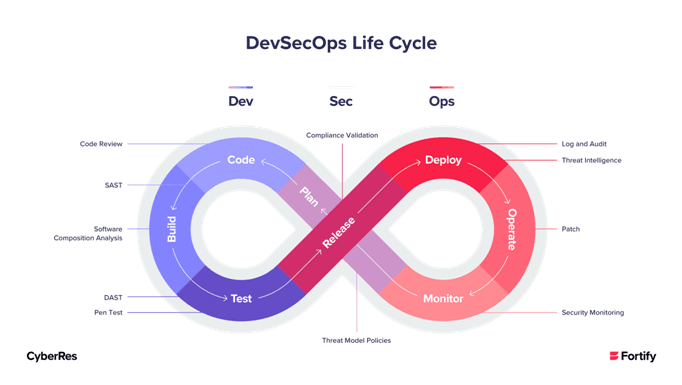
\includegraphics[width=0.8\columnwidth]{Images/devsec.png}
    \caption{DevSecOps Life Cycle}
    \label{fig: DevSecOps Life Cycle}
\end{figure}


\section{Functional Testing vs Security Testing}
Software testing is a very broad area, and each test varies according to its purpose or process - but the primary goal of software testing is to verify the quality of software systems through planned and structured testing under controlled conditions. Functional testing is emphasizing the software's behavior and that the software is working as expected. The functional test cases are based on the requirements of the software which were specified by the stakeholder. There are several functional testing methodologies that can be conducted, such as unit testing and integration testing. White box testing and black box testing are some examples of security testing methods. This topic will be described more in section  \ref{boxtesting}. 
\cite{difftesting} 
Unit testing involves testing small components of the code, which is known as units to determine if the units behave as expected. These tests are typically executed early in the \acrshort{sdlc} to identify bugs early on and save time in the rest of the process. The goal of the unit testing is to run tests on all possible components in an isolated test environment to confirm if the code operates as anticipated. Integration testing, on the other hand, evaluates how the previously tested components perform when integrated into a larger system and communicate across various components. 
\cite{unitvsintergration}

Security testing, on the other hand, wants to break the software to uncover vulnerabilities. The testing aims to identify all possible weaknesses that attackers might exploit. During the testing, the testers perform the test from the attacker's point of view. These kinds of tests can be done manually or be done by software tools, called automated security testing tools. The goal of evaluating security functionalities is to verify if protective measures like authentication are functioning as expected. Security testing will also try to simulate attacks on the software and determine its capability to defend against them.\cite{whysectest}



%Introduction


\section{Application Security Testing}
Application Security Testing can be described as "\textit{process of making applications more resistant to security threats, by identifying security weaknesses and vulnerabilities in source code.}\cite{AST}

Below are some of the different security tools that can be used to make applications more resistant to security threats, and which the group will use in securing the \acrshort{sdlc}. Box testing is also mentioned which is a type of testing technique that the different tools use for testing.  
\newpage
\subsection{Box testing}
\label{boxtesting}

\subsubsection{Black Box Testing}
Black box testing mainly focuses on the functionality and behavior of the application without knowing the structure and processes within it. One can imagine the application being a black box, not being able to see what's inside, but only focusing on the resulting output from the given input. The software will pass the black box test if the input gives the expected output. \cite{blackbox}

\subsubsection{White Box Testing}
White box testing focuses on the application from within. In such tests, the source code and infrastructure will be looked at. The testing consists of covering paths, statements, and branches, among other things. A white box tester looks for security holes by testing the code and therefore requires to have knowledge of programming and IT. The tester looks through the code to find weaknesses such as infinite loops or data flow issues. However, white box testing can be quite complex and when running such testing on a large amount of code, it can take days to test.   \cite{whitebox}

\subsubsection{Grey Box Testing}
Grey box testing is a method that limits the user's knowledge of the different components being tested. It is a combination of white box testing and black box testing, where the user has access to internal code or design but not enough access to run a full white box testing, and the test practices are done at the same level as black box testing. \cite{GreyBox}


\subsection{SAST}
\acrlong{sast} is white-box testing that analysis the source code of an application to identify security vulnerabilities within the code. This method of testing usually takes place during the development phase of the \acrlong{sdlc}. The primary purpose of this method is to identify and remediate security issues before the application actually is deployed. \cite{sast}

\acrshort{sast} tools scan source code for known security threats, such as \gls{Cross-site scripting}, \gls{SQL-injection}, and \gls{Buffer-Overflow}. \acrshort{sast} tools also give warnings on any security weaknesses that may lie in the code that potentially can be exploited. After the tool has gone through the code it generates a report that contains the different vulnerabilities that it has identified, including a more in-depth description of the vulnerability and remediation on how to fix it. \acrshort{sast} usually runs white box testing  which is mentioned in section 2.4.1.2. 

One of the advantages of \acrshort{sast} is that it gives detailed information about the source of the vulnerability, which gives the developer a better understanding of how to fix the issue. 

There are, however, some limitations to \acrshort{sast} tools. For example, it can only detect vulnerabilities that are present in the source code. This means that it cannot detect vulnerabilities that result from the interaction between different components of an application.
\\
\begin{figure}[H]
    \centering
    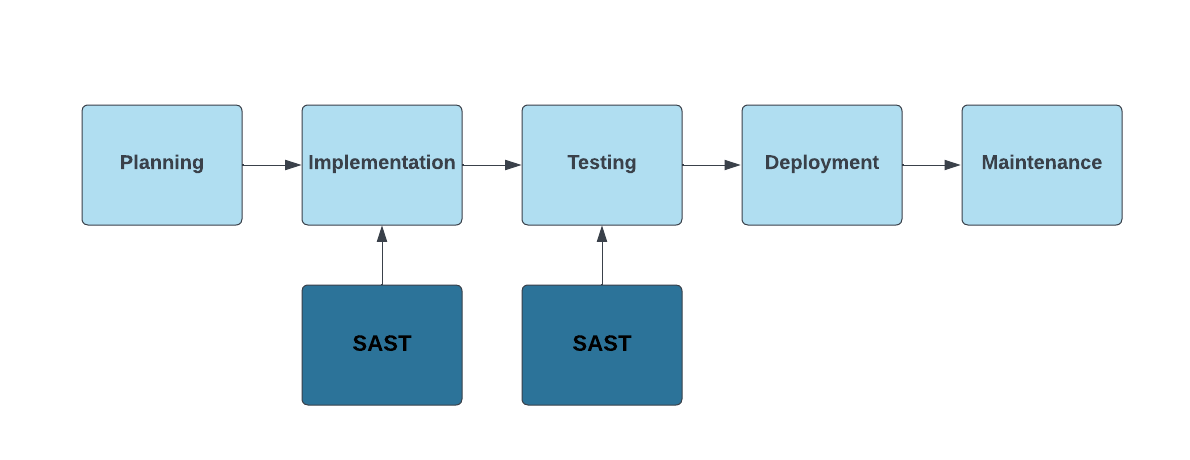
\includegraphics[width=0.8\columnwidth]{Images/sast.png}
    \caption{Where to perform SAST in SDLC}
    \label{fig: Performance of SAST in SDLC}
\end{figure}


\subsection{DAST}
Compared to \acrshort{sast}, \acrlong{dast} is black-box testing. The purpose of \acrshort{dast} is that it evaluates the security of an application by performing security assessments of a running instance of the application. Unlike \acrshort{sast} which analyzes the source code of an application, \acrshort{dast} evaluates the application as its being used, this includes the interaction of different components and the runtime environment. 

\acrshort{dast} simulates real-world attacks, which is done by sending malicious requests and inputs to the application it is testing and then monitoring the responses. In the end, the tool generates a report that includes the different vulnerabilities that were identified, including a more in-depth description as well as remediation on how to fix the issue. 
\acrshort{dast} usually runs black box testing  which is mentioned in section 2.4.1.1. \cite{dast}

An advantage with \acrshort{dast} is that it can identify security issues that are not detectable through \acrshort{sast}, this can for example be interactions between different components. Another advantage is that with \acrshort{dast}, it can identify different vulnerabilities that get triggered, for example when the application is under heavy load or when are specific inputs received.

However, there are some limitations with \acrshort{dast} as well, one being that it can only detect vulnerabilities that are present in the deployed version of the application and cannot give an in-depth description of vulnerabilities that lie in the source code.
\begin{figure}[H]
    \centering
    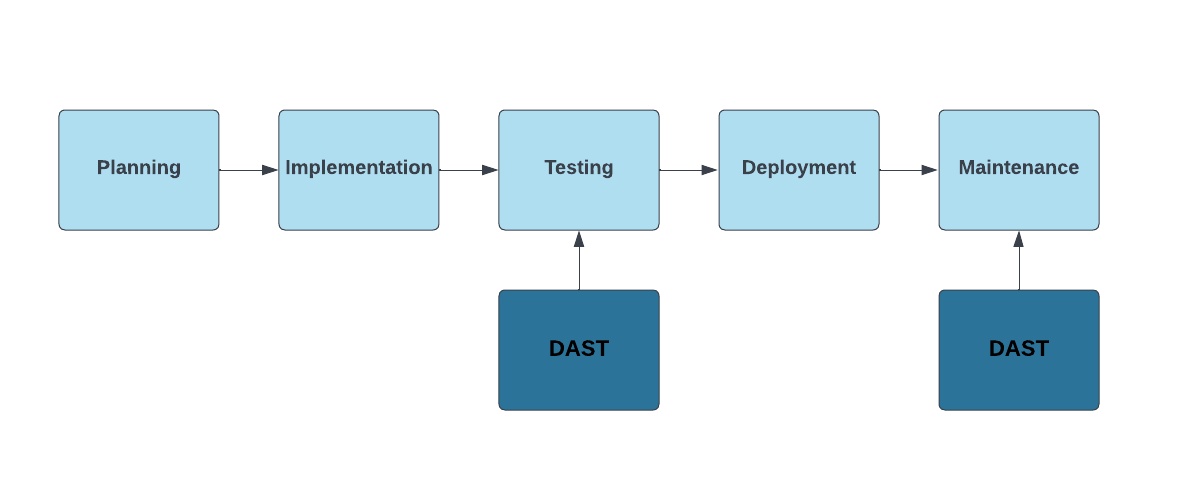
\includegraphics[width=0.8\columnwidth]{Images/dast.png}
    \caption{Where to perform DAST in SDLC} 
    \label{fig: Where to perform DAST in SDLC}
\end{figure}



\subsection{SCA}
\acrlong{sca} is a type of software security testing tool that analyzes the dependencies of a software application to identify and manage potential security risks. The main objective of the \acrshort{sca} is to identify third-party components that may contain security vulnerabilities. \cite{sca}

 \acrshort{sca} scans the application's code to identify all of its \gls{dependency}, including the different versions of the components used. It then cross-references these \gls{dependency} to different databases that include known vulnerabilities and then generates a report containing any potential risk. In comparison to the others, the report also includes an in-depth description of the vulnerability as well as a recommendation to update the components to newer versions or replace these. \acrshort{sca} usually runs grey box testing  which is mentioned in section 2.4.1.3. 

An advantage with \acrshort{sca} is that it can quickly identify risks that may be introduced from third-party components. It is rather common that modern applications rely on a large number of different dependencies, which therefore make \acrshort{sca} useful. It can provide a comprehensive view of the security risks associated with an application and help developers make informed decisions about the security and their applications. 

However, it is important to remember that \acrshort{sca} does not always have access to updated information, and may give some false positives about vulnerabilities that don't necessarily exist anymore. 
\\
\begin{figure}[H]
    \centering
    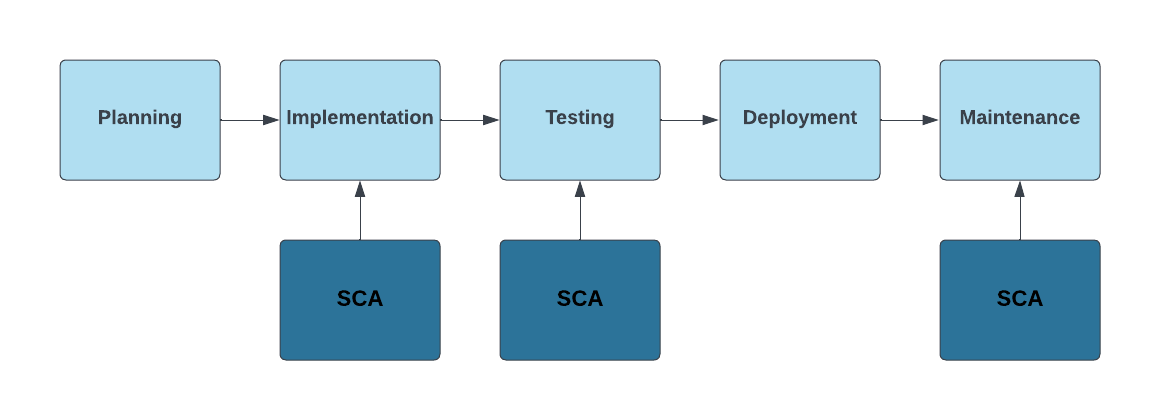
\includegraphics[width=0.8\columnwidth]{Images/sca.png}
    \caption{Where to perform SCA in SDLC} 
    \label{fig: Where to perform SCA in SDLC}
\end{figure}

\newpage
\subsection{Comparison of SAST, DAST, and SCA}
Upon reviewing the different security application tests, similarities between \acrshort{sast}, \acrshort{dast} and \acrshort{sca} were discovered. The table below shows some commonalities, which indicates that a combination of the different testing mechanisms can enhance the testing process of the application. 
\begin{figure}[H]
    \centering
    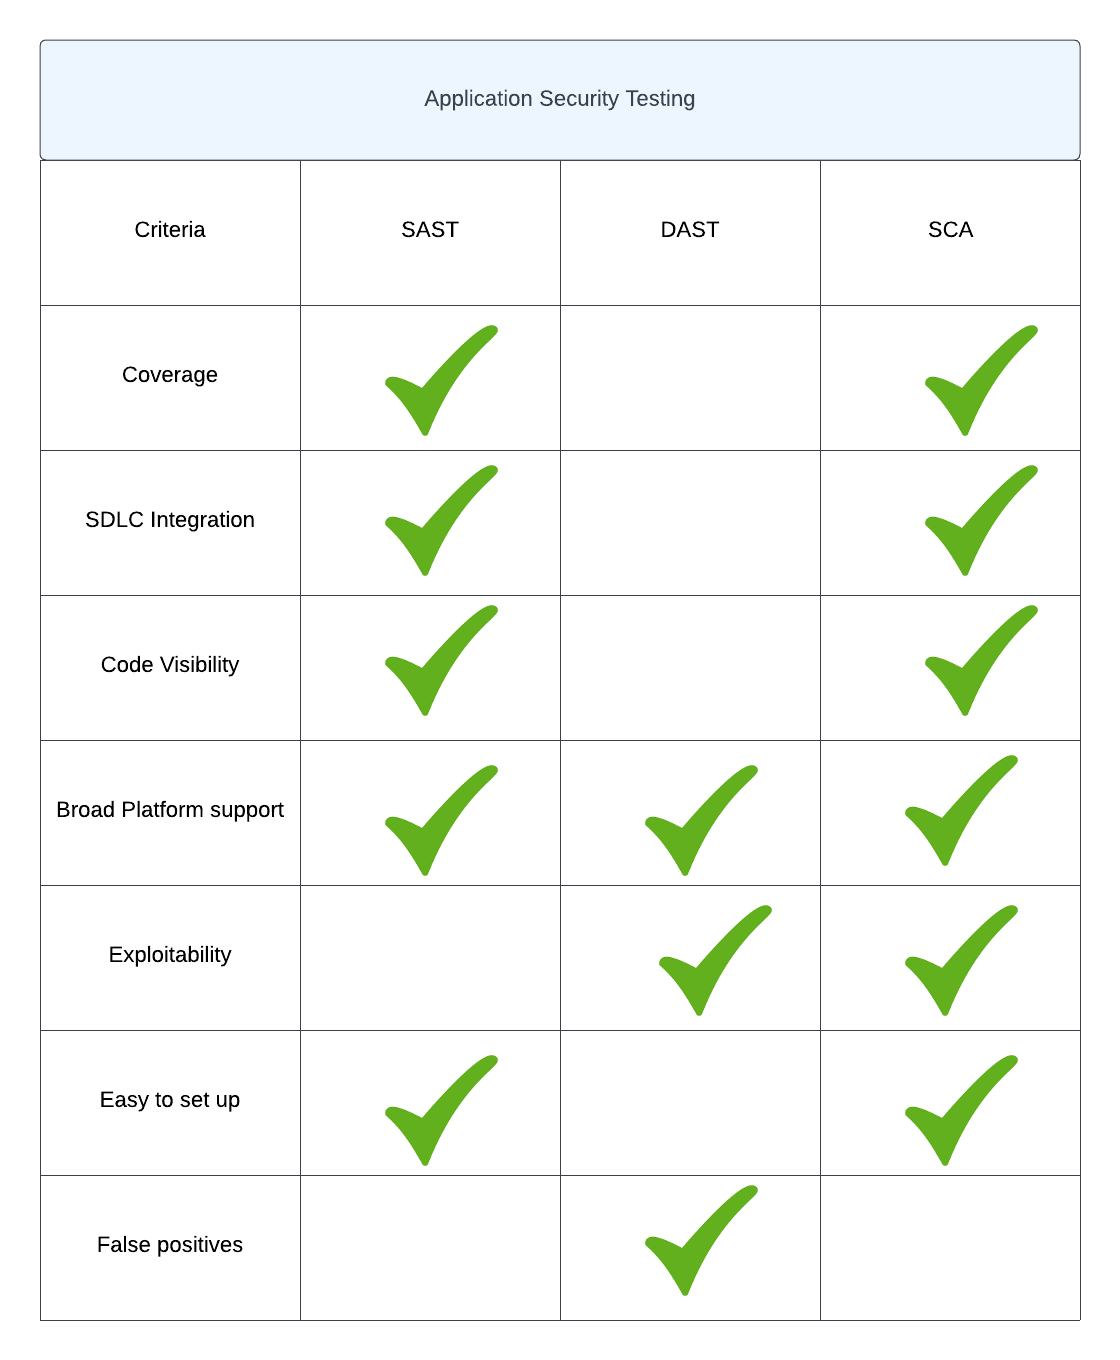
\includegraphics[width=0.8\columnwidth]{Images/ApplicationSecurityTesting.png}
    \caption{Comparison of SCA, DAST, and SAST}Adapted from: \cite{Comparison}
    \label{fig: Comparison of SCA, DAST, and SASt}
\end{figure}

\newpage
\section{The Significance of Software Security Testing}
Security testing plays a critical role in the \acrlong{sdlc}, as it is employed to identify potential security vulnerabilities in the system and prevent real-world attacks. It is a process where the security of the system is evaluated and identifies the system's possible security weaknesses and risks of vulnerability.\cite{whysectest}

According to IBM's report, in 2022, the cost of a data breach was estimated to be USD 4.35 million\cite{databreach}. Investing in cybersecurity measures can potentially save a lot of money for a company in the event of a cyber attack. The report states that companies that have implemented zero trust security measures saved about USD 1 million in breach costs on average when compared to those that have not. To repair a vulnerability in the design phase costs an average of USD 500\cite{fixvulnerability}. Starting software testing early in the SDLC results in reduced costs and saved time. 

As mentioned in section 2.3, there are various types of testing that should be executed on an application, including testing of both the written code and the libraries that are integrated and being used. It is crucial to test libraries because they can contain various types of vulnerabilities, especially if they are open-source. This is because open-source code is open to common vulnerabilities, which can expose the application to malware injections, distributed denial-of-service (DDoS) attacks, and exposure of sensitive data. \cite{testlibaries}

\section{OWASP Top 10}
\acrlong{owasp} (\acrshort{owasp}) serves as a standard reference document for web application security and developers to raise their knowledge of potential security threats. It represents an agreement on the most critical threats to web-based applications. The document contains a prioritized list and recommendations for fixing the 10 severe security flaws in web applications. The function of this article is to educate readers on the most common safety risks that may occur. Developers and security professionals may use this knowledge and implement it into their security policies, reducing the frequency of these dangers in their applications. 


\section{Vulnerability Risk Rating}
Discovered vulnerabilities can be rated by standardized systems like CVSS, CVE, CWE, and OWASP Risk Rating Methodology. These databases are frequently used in application security testing, particularly in SCA scans, to uncover code patterns that may indicate a common vulnerability within the code. While they may also be utilized in DAST and SAST scans, they are most commonly used in SCA scans. 

\subsection{Common Vulnerability Scoring System (CVSS)}
\acrlong{cvss}, known as \acrshort{cvss}, is \textit{"a Security Content Automation Protocol (SCAP) specification for communicating the characteristics of vulnerabilities and measuring their relative severity"}\cite{nistCVSS}. The system is used to give vulnerabilities a numeric score based on their severity. The scores can be translated into low, medium, high, and critical to assist organizations to evaluate and rank their vulnerabilities. CVSS is currently at version 3.1. \cite{CVSS}
\begin{figure}[H]
    \centering
    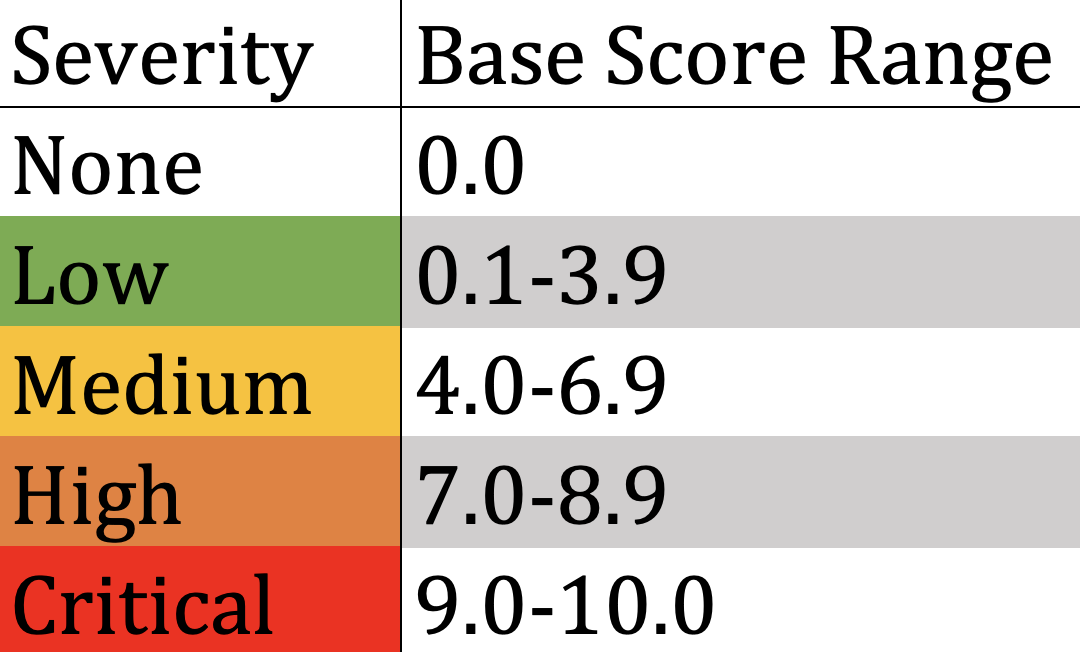
\includegraphics[scale=0.3]{Images/CVSS.png}
    \caption{CVSS v3 Ratings} Adapted from:\cite{cvssrating}
    \label{fig:CVSS v3 Ratings}
\end{figure}


\subsection{Common Vulnerabilities and Exposures (CVE)}
\acrlong{cve}\footnote{Available at: https://www.cve.org/}, known as \acrshort{cve}, is, according to their website,\textit{"a list of records each containing an identification number, a description, and at least one public reference for publicly known cybersecurity vulnerabilities"}\cite{CVE}. The CVE program's mission is to determine, describe, and categorize cybersecurity vulnerabilities that have been made public. All discovered vulnerabilities will be put into records and sent to NVD.

\subsection{Common Weakness Enumeration (CWE)}
\label{cwe}
\acrlong{cwe}\footnote{Available at: https://cwe.mitre.org/}, know as \acrshort{cwe}, is \textit{"a community-developed list of common software and hardware weakness types that have security ramifications"}\cite{CWE}. It was established to serve as a consistent benchmark for security solutions that address vulnerabilities and as a baseline for identifying, mitigating, and preventing weaknesses. CWE's goal is to provide instructions for those who have control over and maintain source code to stop the vulnerabilities at the source. 

\subsection{OWASP Risk Rating Methodology}
OWASP Risk Rating Methodology contains a formula that calculates a risk score for each vulnerability based on two factors: likelihood and impact. There are multiple factors that make up both likelihood and impact. 
 
Factors that together compose the estimation of likelihood are separated into different groups which are related to the threat actor and the vulnerability. The set of factors related to the threat actor is skill level, motive, opportunity, and size. The set of factors related to the vulnerability is the ease of discovery, ease of exploit, awareness, and intrusion detection. Each factor will have different options, and each option will receive a likelihood rating from 0-9. 

Factors that together compose the estimation of impact are divided into technical impact and business impact. The technical impact is broken down into confidentiality, integrity, availability, and accountability. Further, the business impact is divided into financial damage, reputation damage, non-compliance, and privacy violation. All of the factors will, like the factors of likelihood, receive an impact rating from 0-9. 

Combining the estimates of likelihood and impact factors produces an overall severity level of the risk, which can be classified as low, medium, or high (as shown in Figure 2.5) in order to determine its severity. These levels can be further combined to determine the final severity of the risk, as illustrated in figure 2.6.\cite{owasprisk}

\begin{figure}[H]
    \centering
    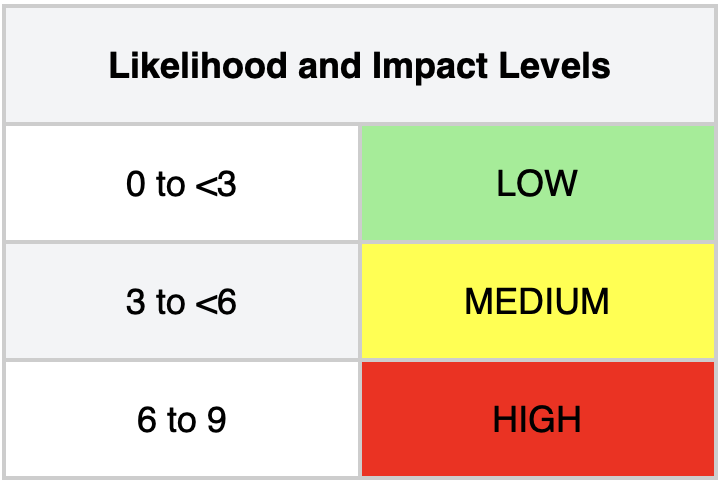
\includegraphics[scale=0.5]{Images/OWASP-likelihood.png}
    \caption{The likelihood and impact levels}
    \label{fig: Impact levels}
\end{figure}

\begin{figure}[H]
    \centering
    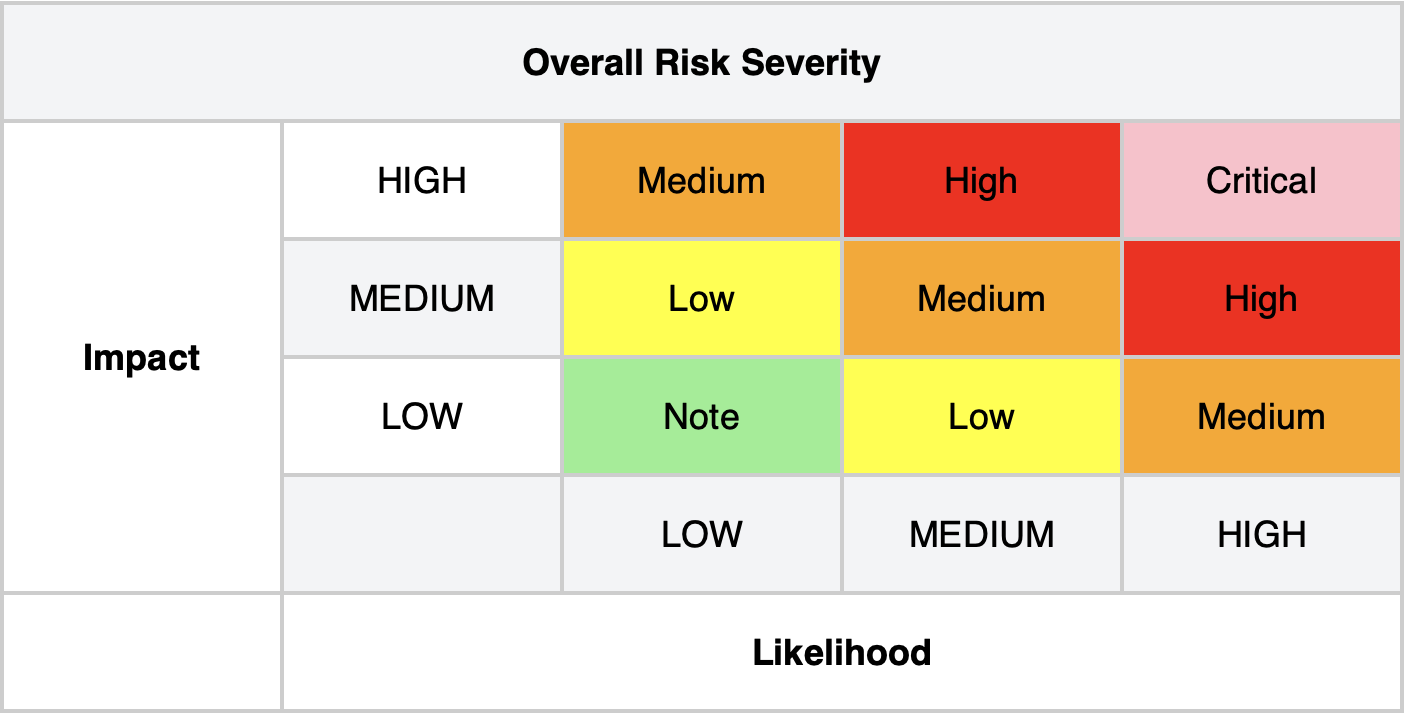
\includegraphics[scale=0.4]{Images/OWASP-severity.png}
    \caption{Severity level based on impact and likelihood}
    \label{fig: OWASP Severity Scale}
\end{figure}
\newpage




\section{Amazon Web Services}
\acrlong{aws}\footnote{Available at: https://aws.amazon.com/}, known as \acrshort{aws}, is a cloud computing platform distributed by Amazon and provides a range of services from \acrlong{iaas}(\acrshort{iaas}) to \acrlong{paas}(\acrshort{paas}), and everything in between, allowing customers to run their applications and store their data in the cloud. With their pay-as-you-go cloud computing model, the customer can scale their resources up and down - without having to invest in physical infrastructure.\cite{aws}  

\section{GitHub}
GitHub\footnote{Available at: https://github.com/} is a web-based software development platform where developers can collaborate and store open-source projects. The developers can manage their projects in repositories, and track bugs and issues. It offers a range of different collaboration tools, including pull requests, code reviews, and project management functionalities. Git is a version control system, utilized for the management and monitoring of file versioning. GitHub employs this technology as the basis for its service. This allows developers to work on code simultaneously, track changes, and merge contributions from multiple contributors.\cite{github}

\newpage
\input{BachelorThesis/3-Security Tools For The Pipeline}
\newpage
\chapter{Analysing of tools}
\section{Introduction}

\section{GPG vs. SSH keys for signed commits}

\definecolor{lightblue}{RGB}{176, 222, 241}

\begin{table}[!ht]
    \centering
    \begin{tabular}{|p{0.4\textwidth}|p{0.4\textwidth}|}
    \hline
        \cellcolor{lightblue!} GPG keys  & \cellcolor{lightblue!} SSH keys \\ \hline
        Not that hard to configure?? &  Not that hard to configure??\\\hline
        Encrypts data &\\ \hline
        Public key for encryption &\\ \hline
        Private key for decryption &\\ \hline
        \acrshort{idea} for data encryption &\\ 
    \end{tabular}
    \caption{GPG vs. SSH keys}

\end{table}

\section{CodeQL}
Postive: For free! Open source, easy to configure, integrated into github
\\
Negative: Open source (everyone can edit)
\\
CodeQL and Dependabot have together detected 101 vulnerabilities. This is the exact amount of vulnerabilities that was "...intentionally planted in the application..." \cite{owaspJuiceShop}.

\section{Dependabot}


\newpage
\chapter{Security in the pipeline vs security of the pipeline}














\section{Security in the pipeline}
Security in the pipeline is the process of implementing different measures and controls to protect the code that is being sent through the pipeline from various security threats. The pipeline commonly consists of multiple phases like code development, testing, and deployment, all of which may be susceptible to various security threats, like unauthorized access, data breaches, malware, and denial-of-service attacks. Security in the pipeline is crucial to secure the integrity and confidentiality of software applications and data.

\subsection{Code Scanning}
%du tester koden som skal bli deployet, alstå det som ligger inni pipelinen. Sjekkes for sårbarheter etc
Code scanning is security measure where you analyze the code with the help of a tool to find security vulnerabilities and coding errors. Code scanning serves as a preventive measure against developers introducing new issues. During this step, you can perform a SAST scan using specialized tools that are designed to scan through code. 
\\~\\
GitHub has an integrated code scanner called CodeQL. When using this code scanner, it extracts all source code into a relational database made for CodeQL, which is analyzed by running queries against it to identify vulnerabilities and insecure patterns. The user can either take advantage of the large quantity of queries already made by other developers, or they can make their own. An example of a simple query could be getting the location of all method calls in the code. 
 \cite{codeql}
\subsection{Scan Dependencies and Open Source Libraries}
All dependencies, open source libraries and third party artefacts that has been utilized should be validated. This can be done by checking their checksum against a reliable, good source and validating any cryptographic signatures. If any third party software was implemented in the application it's important to conduct an SCA scan using suitable tools to identify whether any vulnerable open-source software was used. \cite{bestpracticeSupplyChain}

\subsection{Secret Scanning}
To prevent or identify accidental exposure of "secrets", like access tokens, SSH keys, or other credentials, one should execute a secret scanning on a Git repository. Secret scanning tools, such as GitHub's secret scanning, can be used to find these vulnerabilities, and alert developers to potential security risks. \cite{GithubSecretScanning}

\subsection{Dynamic testing}
In software best practices, it is recommended to run multiple tests and scans to identify bugs and errors - where one of these tests is \acrlong{dast} (\acrshort{dast}).\cite{bestpracticeSupplyChain} This sort of scan tries to penetrate the application, attempting to identify vulnerabilities and weaknesses in it. One can implement a tool specialized for DAST scans, such as XX, which can identify security risks like cross-site scripting, SQL injection or path traversal.\cite{dynamictesting}


\subsubsection{The Limitations of DAST Tools}
Even though \acrshort{dast} can be used to identifying potential vulnerabilities, there are certain types of threats that may go undetected. For this reason, the company should engage a red team, which is a group of experts capable of performing penetration testing. A pen test will provide a more realistic test, as it simulates a real-world attack, detects more complex vulnerabilities and provide a more comprehensive view of an application's security posture. A pen test can also function as a validation of the \acrshort{dast} scan, as it can help determine if the vulnerability can be exploited and the potential impact of the vulnerability. \cite{dastpentesting}




\newpage
\section{Security of the pipeline}
Security of the pipeline in short terms are the security measures that are taken into consideration when securing the pipeline itself. This includes not only securing the pipeline istelf, but also the infrastrucutre, components, network that are used to process the code that goes through the pipeline. Securing of the pipeline ensures that the code is not tampered through during the process of going through the pipeline. 

\subsection{Signed Commits}

\subsection{Branch Protection}

\subsubsection{Require a pull request before merging}
Administrators of the repository can add rules to the repository which restricts pull requests to have a specific number of people approving the changes before merging to a protected branch. Administrators can allow users with written permissions to do the approving as well as users considered to be code owners. \cite{ProtectedBranches}

It is under this type of protection the "four eyes" principal is applied. Since this type of protection require that at least two people approve the merge, this includes the person itself doing the changes, this principal is a controling mechanism that increases the security measures. 
\subsubsection{Require status checks to pass before merging}
hei
\subsubsection{Require conversation resolution before merging}
hei
\subsubsection{Require signed commits}
hei
\subsubsection{Require linear history}
hei
\subsubsection{Require deployments to succeed before merging}
hei
\subsubsection{Lock branch}
hei
\subsubsection{Do not allow bypassing the above settings}
hei

\newpage



\subsection{Access Control}
\subsection{File Storage and Preservation}

\newpage
\chapter{Deployment}
\section{Introduction}
\section{Code used in the pipeline}
For testing the group decided on using OWASPs Juice Shop, which is a deliberately vulnerable web application that is designed to help developers and others to learn about web applications security concepts. The code is designed to simulate a real-world application by having common vulnerabilities within the code. The intention is to encourage users to find these vulnerabilities and to exploit them and increase the understanding of web application security \cite{owaspJuiceShop}.
The code in the OWASP Juice Shop is open source code on GitHub and is written in TypeScript, which uses a Node.js server and Angular for front-end. \cite{owaspJuiceShopCode}
The code contains of different vulnerabilities, including SQL injections, cross-site scripting and many others. 
Overall, OWASP Juice Shop encourages users to improve their skills and it allows for customization and adaption for specific needs from the users. 


\section{Security when coding}
Here we can write something about security while coding, maybe get CodeQL to work so we can test that idk??? Maybe out of scope

\section{Security when pushing to GitHub}

\subsection{Access control}
Something about access control

\subsection{Branch protection}
Can easily be enabled in GitHub. 

\subsection{Signed commits}
Generate a SSH or a GPG key. Connect it to your GitHub account. Let the wanted repository know you want to use a given key for signing, and sign off on every commit. This secures the authentication of the commiter. 

\section{Security when in Git}
Code scans, dependabot and secret scanner needs to be enabled. Dependabot only needs to be enabled, and does not require any configuration. 

\subsection{Configuring CodeQL}
When configuring CodeQL in a GitHub repository, one can either use a default setup or configure it themselves. 

\subsection{Dependabot}

\subsection{Secret Scanning}


\section{AWS}
\subsection{Terraform}
Terraform is a tool for automating resource configurations. In this case, Terraform is used to configure the AWS CodePipeline. \\
Write about automation, idempotent etc.. \\
In the code: specifies git repo, write build commands, apply it \\
Include code snippets?

\subsection{Signed Artifacts}


\subsection{OWASP Zap}


\subsection{Penetration testing}

\section{Security after deployment}
\newpage
\chapter{Testing}
\section{Introduction}

\section{Testing environment}

\subsection{Amazon Web Services}
\acrlong{aws}, known as \acrshort{aws}, is a cloud computing platform distributed by Amazon and provides a range of services from \acrlong{iaas}(\acrshort{iaas}) to \acrlong{paas}(\acrshort{paas}), and everything in between, allowing customers to run their applications and store their data in the cloud. With their pay-as-you-go cloud computing model, the customer have the ability to scale their resources up and down - without having to invest in physical infrastructure.\cite{aws}  

\subsection{GitHub}
GitHub is a web-based software development platform where developers can collaborate and store open-source projects. The developers can manage their project in repositories, and track bugs and issues. It offers a range of different collaboration tools, including pull requests, code reviews, and project management functionalities. Git is a version control system, utilized for the management and monitoring of file versioning. GitHub employs this technology as the basis for its service. This allows developers to work on code simultaneously, track changes, and merge contributions from multiple contributors.\cite{github}

\newpage
\chapter{Discussion}
\section{Introduction}
This is another test \cite{nbimattacks}

\section{Chosen branch protection rules}
When deciding which branch protection rules to implement, it is important that securing the branch does not drastically affect the work flow. There are several possible protection rules to enable, described in \ref{branchprotection}. Though, enabling all of the rules at once may do more harm than good, as every pull request and commit must go through several steps which will make the work flow less efficient. Therefore, selecting only the most useful rules will benefit the development. 
\\~\\
The "Four Eyes Principle" is a mechanism where activities, in this case pull requests, needs approval from two individuals.  This principle is implemented by enabling "Require a pull request before merging", and require two approvals before merging. By enabling this rule, the risk of unwanted code being merged into the basecode is lower, without disrupting the work of all developers since only two need to look through the code. \cite{foureyes}
\\~\\
Another implemented branch rule, is requiring signed commits. Signed commits requires some pre-configurations, but once that is done, all the developers have to do is enter a passphrase, and the commit is verified. By implementing required signed commits, it ensures the integrity of the code while the work flow undisturbed.

\section{Chosen SAST tool}
\newpage
\newpage
\thispagestyle{empty}
\mbox{}

\chapter{Conclusion}
\section{Introduction}
This chapter includes a discussion of the work done, the techniques employed to achieve the intended outcomes, and several constructive suggestions to enhance the quality of the thesis.

\section{The Work Process}

\subsection{Meetings}
The team held meetings with their supervisor, Filip Holik, every week. Although the meetings were typically scheduled for Wednesdays, they had to be postponed or canceled on occasions due to various circumstances. Meeting Minutes with the supervisor can be found in Appendix \ref{supervisormeeting}.
\\~\\
During the early stages of the project, the team met with the stakeholder every other week. However, as the project progressed, both parties agreed that weekly meetings would be beneficial. In addition, as the demand for help grew, the group required more regular assistance. Meeting Minutes with the stakeholder can be found in Appendix \ref{nbimmeeting}.  

\subsection{Scrum}
Throughout the thesis, the group followed the Scrum framework of agile project management, which required breaking the project into sprints lasting two to four weeks. Daily stand-up meetings were held to keep everyone informed, during which members delivered progress reports on the thesis and discussed plans for the day, including each member's allocated chores. While the group aimed to meet daily, this was sometimes difficult to achieve as some members had work obligations besides their studies.
\\~\\
Despite this, the team had sprint planning and retrospective sessions every two weeks to review progress and establish goals for the next two weeks. During the retrospective meetings, the team engaged in self-reflection by asking questions such as \say{What should we keep/stop doing?}, \say{What should we do more/less of?} to identify improvement areas for the next sprint cycle. During the sprint planning meetings, on the other hand, the group evaluated completed tasks and discussed what needed to be done before the next sprint period.
\\~\\
Following the Scrum framework helped promote good communication and teamwork among group members. Furthermore, the Kanban board was integrated into the Scrum Framework and proved to be quite helpful in tracking tasks that were ongoing, completed, or yet to be started. 

\subsection{Coordinated schedule}
In order to better coordinate their busy schedules, group members with different commitments, such as work and student associations, decided to implement a scheduling method. Doing this allowed them to quickly determine each other's availability and schedule meetings more efficiently. To achieve this, the team utilized the calendar feature within their Teams channel to schedule their activities and workdays.

\subsection{Draft Submissions}
The team set specified deadlines for producing multiple drafts at the start of the project. This approach tried to maintain constant development while avoiding last-minute delays. For instance, the group set an April 3rd target for their first draft, which they could meet. As a result, both the supervisor and the stakeholder received the first draft on time. After a few days, the team got feedback and proceeded with their work accordingly. 
\\
Additionally, the group established a deadline for the final draft. Setting the final draft deadline on the 1st of May, three weeks before the submission date of the 22nd of May, gave the stakeholders and supervisor sufficient time to review the thesis thoroughly. It is essential to mention that the group followed the plan comprehensively, allowing them to send in multiple drafts for review and refinement before the final submission. 


\subsection{Gantt Chart}
Since the group decided to change the scope during the project period, the original Gantt chart could not be followed. 
\\~\\
The research on tools was initially considered time-consuming, but with the changes made, this activity became a minor part of the thesis than anticipated. As a result, it took less time than what was first estimated. Furthermore, the \say{Testing tools} activity was removed since the team wanted to focus less on testing tools and more on integrating testing of the various tools into the pipeline-building process. 
\\~\\           
The process of learning \acrshort{aws} and configuring the pipeline with Terraform took more extended time than initially expected.
The documentation for \acrshort{aws} and Terraform is extensive, but navigating it can be overwhelming. With so many different services and features offered by \acrshort{aws}, the group had to determine the best fit for their needs. In addition, building the pipeline required a significant amount of functionality to be in place for additional features to work correctly. 
\\~\\
However, the group followed the scheduled deadlines for the various draft submissions. Consequently, the initial draft was submitted on April 3rd in week 13, but after discussions with the supervisor (see meeting minutes in Appendix \ref{ChangeFinalDraftDateMeeting}), it was requested to be rescheduled to May 5th in week 18, resulting in additional work being accomplished within those two days.

\vspace{2mm}
\begin{figure}[H]
    \centering
    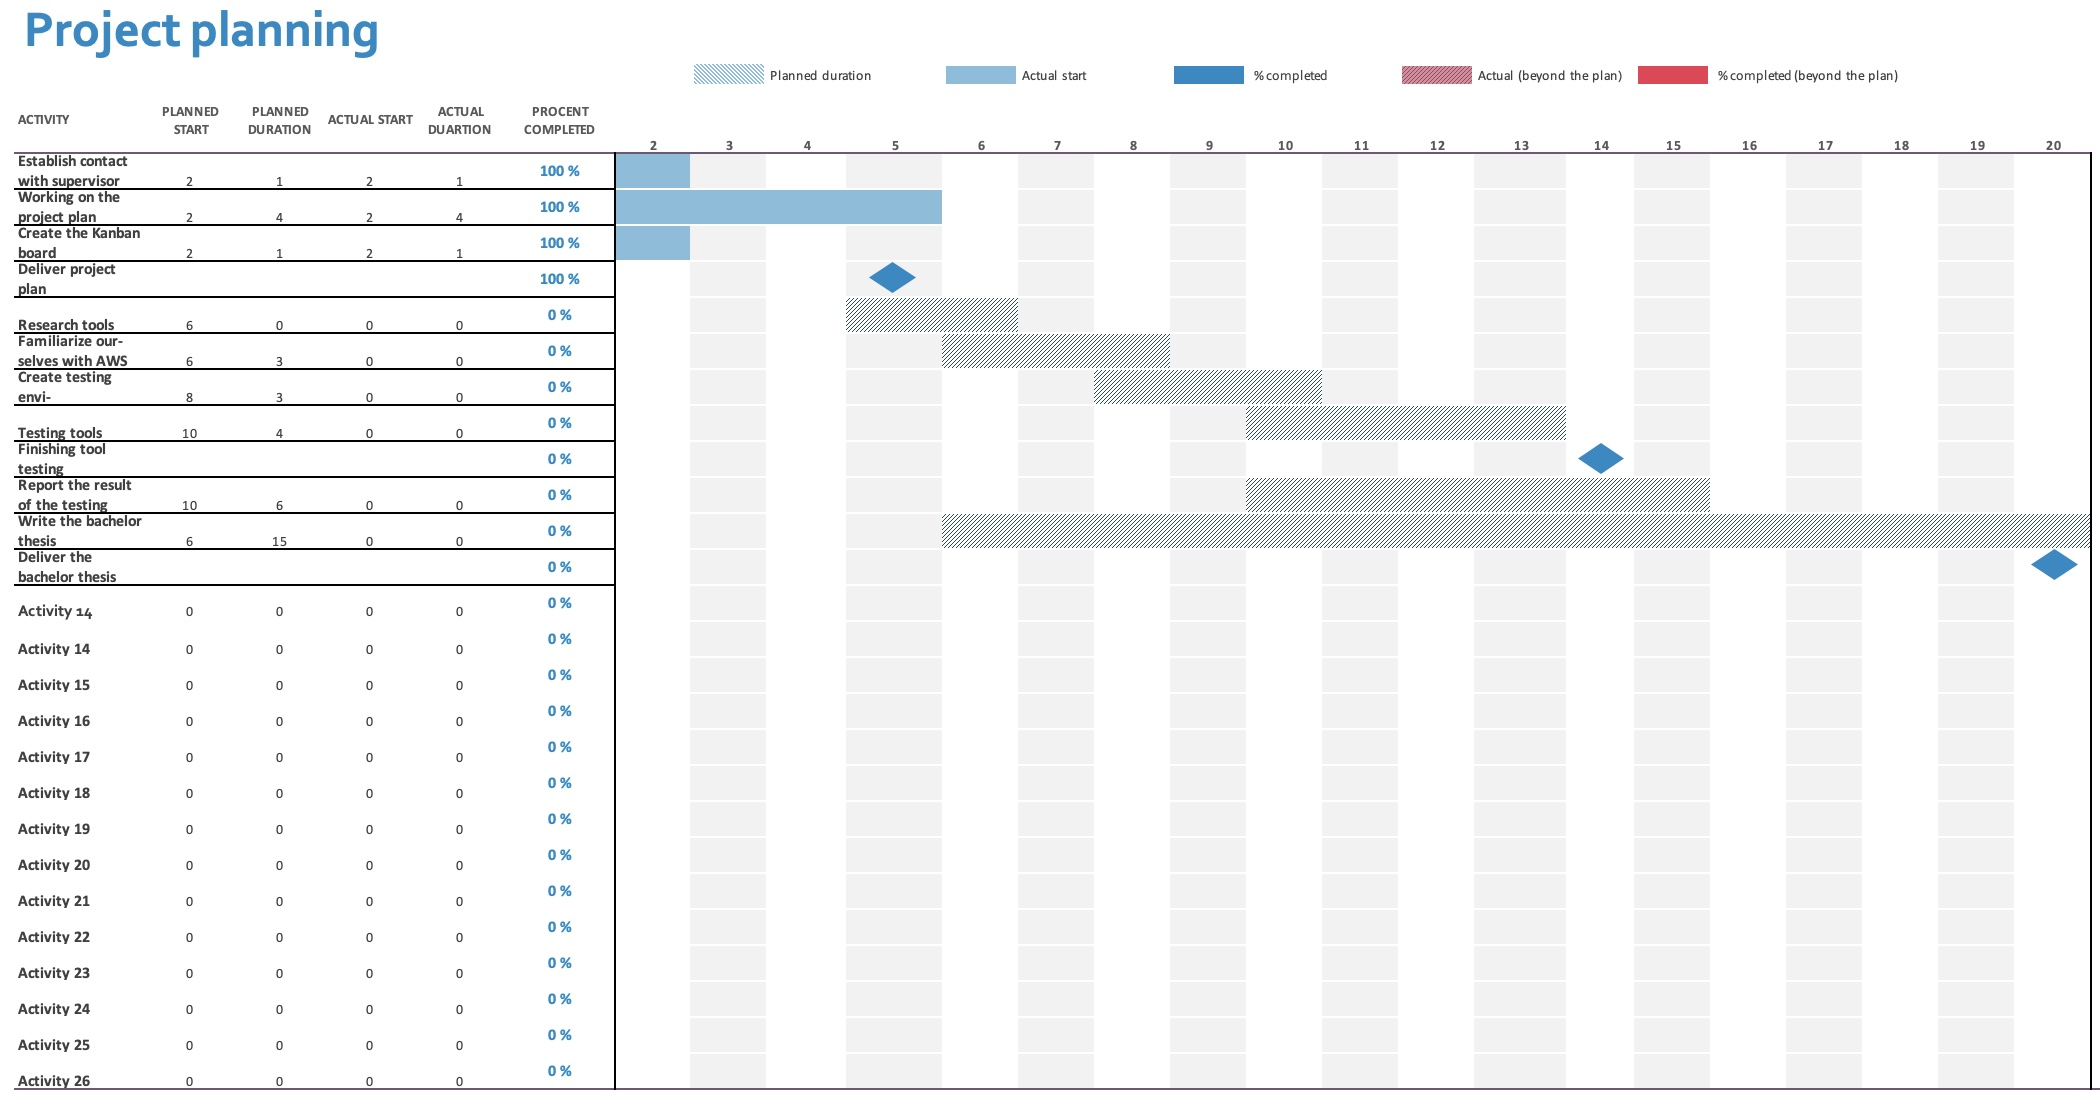
\includegraphics[width=1\columnwidth]{Images/gantt2.jpg}
    \caption{Original Gantt Chart}
    \label{fig: Original Gantt Chart}
\end{figure}

\vspace{2mm}
\begin{figure}[H]
    \centering
    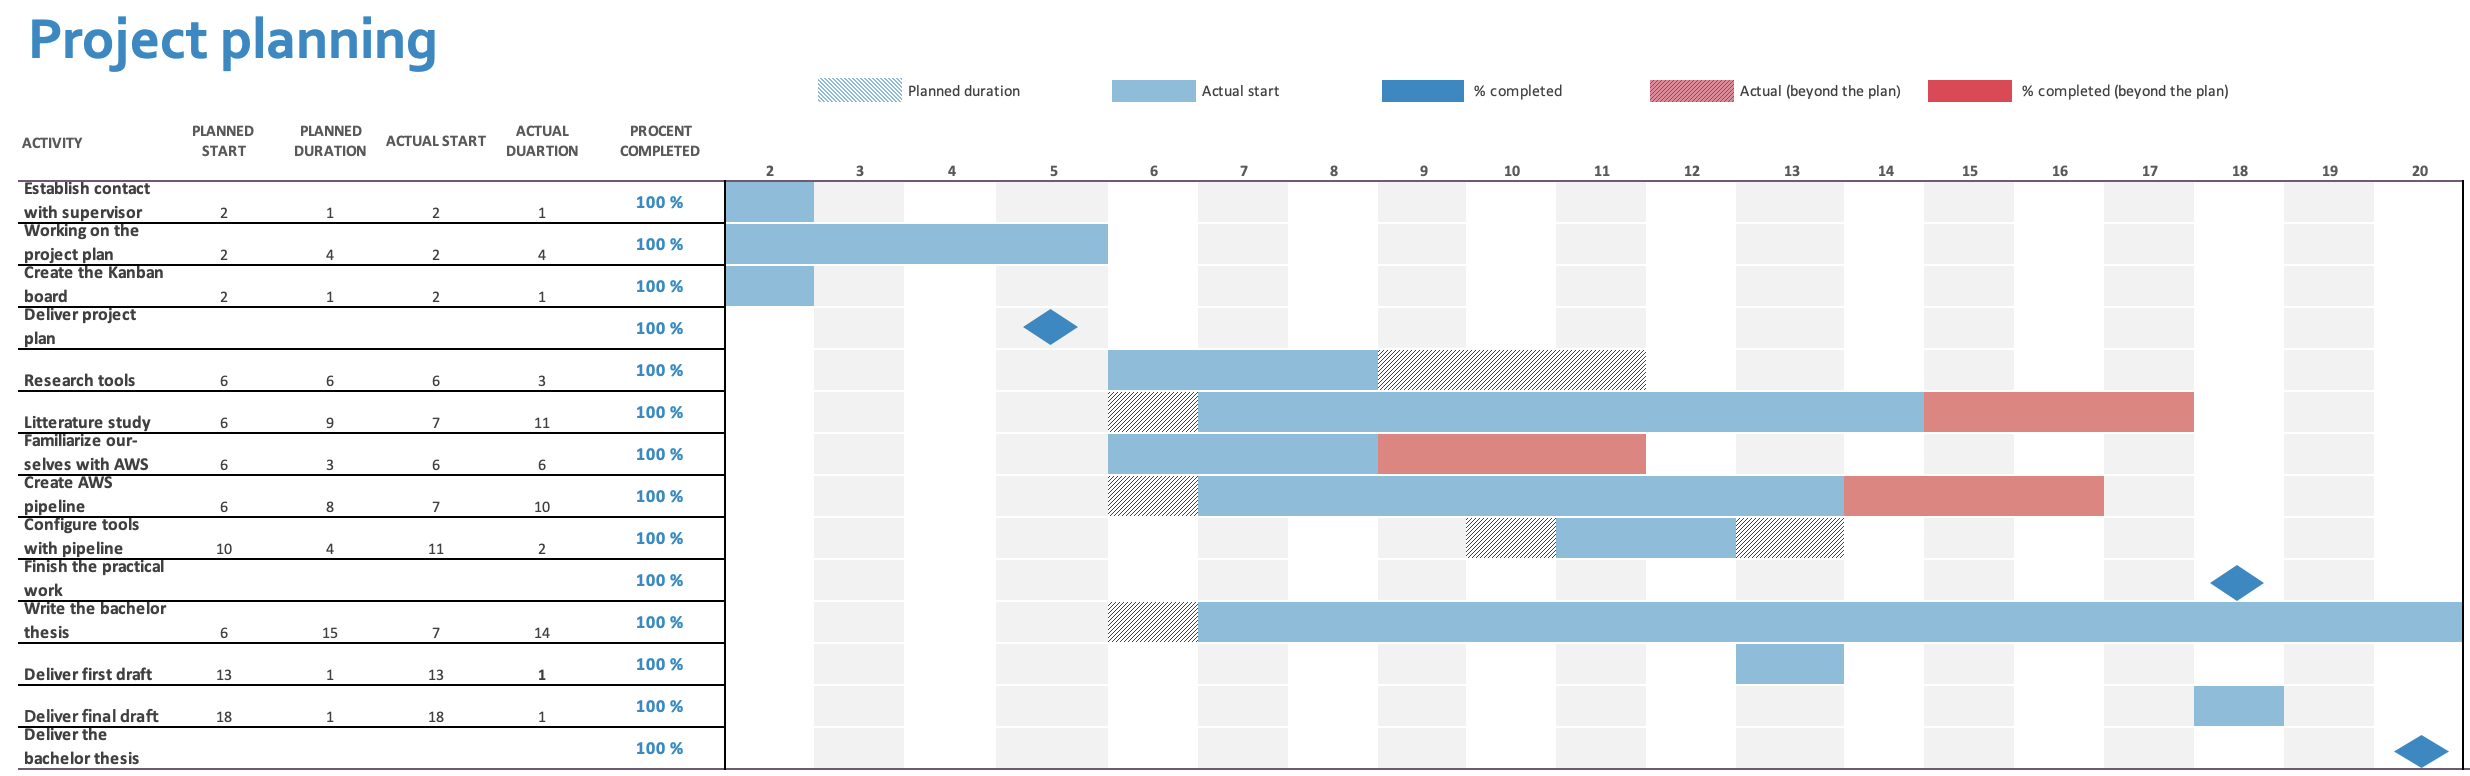
\includegraphics[width=1\columnwidth]{Images/finished-gantt.png}
    \caption{Updated Gantt Chart}
    \label{fig: Updated Gantt Chart}
\end{figure}


\subsection{Distribution of Work}
The group decided to divide the work into two parts at the start of the thesis to ensure that the thesis progressed continuously. The first part is practical, and the second is report writing. The responsibilities were assigned based on each group member's strength and what they most desired to do. As a result, every group member contributed to the thesis, and everyone worked together to complete the report on time. 

\subsection{Goals}
P1: \textit{Collaborate effectively with team members to ensure the timely completion of tasks} was achieved. As stated previously, the group incorporated a Kanban board into the Scrum framework allowing for the assignment and tracking of tasks. Additionally, the group utilized various communication platforms, such as Discord and Teams, to ensure effective communication among the group members. Using communication tools already integrated into each member's daily workflow was essential, and these two platforms proved to be the most effective for the group's needs. 
\\~\\
P2: \textit{Successfully integrating security tools (e.g., \acrshort{sast}, \acrshort{dast}, \acrshort{sca}) into the \acrshort{sdlc} \gls{pipeline}} was achieved. The group found tools that could be integrated into the \gls{pipeline} between GitHub and \acrshort{aws} to secure the application code being sent through.
\\~\\
P3: \textit{Implement an automated \gls{pipeline} using Terraform to build, test, and deploy applications} was achieved. The group created Terraform code that automated the pipeline from the build to the deployment. 
\\~\\
R1: \textit{Develop a secure and automated \gls{pipeline} for the \acrshort{sdlc} process using Terraform}, is partially achieved. The group developed an automated pipeline using Terraform code and implemented restricted access management to ensure pipeline security. However, it would be overly confident to claim that the \gls{pipeline} is 100\% secure, as the group did not have sufficient time to implement signed artifacts. This would have ensured that the code pushed to the GitHub repository was the same as the code sent through the \gls{pipeline}, thus guaranteeing code integrity. Consequently, while the \gls{pipeline} can be deemed secure, the group cannot be entirely specific that the code sent through is secure. Hence, the goal of achieving a complete, secure, and automated \gls{pipeline} remains partially fulfilled. 
\\~\\
R2: \textit{Produce a report summarizing the project results and recommendations for improving the \acrshort{sdlc} \gls{pipeline} security}, was accomplished. The resulting report provides numerous essential and effective practices that can be implemented to improve security in the \acrshort{sdlc}, and the goal was achieved within the requirements given. 

\section{Further Work}
For further work, the thesis could be strengthened by performing a broader analysis of various security tools that perform \acrshort{sast}, \acrshort{dast}, and \acrshort{sca} scans -  where the selected tools are based on these analyses. During these analyses, an assessment can also be made of which requirements must be met for a tool to be selected. 
\\~\\
Including earlier phases in the thesis would have been beneficial to acquire a more thorough grasp of the entire \acrlong{sdlc} and adhere to the shift-left methodology, which emphasizes early testing to find vulnerabilities earlier.   
\\~\\
%Despite successfully automating most of the \gls{pipeline}, the group encountered challenges in automating Secret Scanning in GitHub. The lack of documentation on enabling it through \acrshort{cli} or Terraform code limited the progress. Consequently, the group prioritized other tasks and allocated more time to this aspect in future work. The ultimate goal remains to achieve a fully automated \gls{pipeline}. 

%Write about code integrity!!!! NEED MORE OF THIS!

\section{Conclusion}
The group is pleased to state that they have completed their thesis project, meeting the requirements set by their stakeholder while staying within the project's scope. The input from the stakeholders was critical in determining the group's objectives and requirements, resulting in a successful outcome that met the expectations of everyone involved.
\\~\\
After careful consideration, the group recommends developers to implement \acrshort{sast}, \acrshort{sca} and secret scanning in the implementation phase of the \acrshort{sdlc}. Further, they recommend 



the group found that integrating Dependabot and CodeQL on GitHub was the most viable option in regards to using \acrshort{sca} and \acrshort{sast} tools. The implementation process was smooth, and the group encountered no significant issues throughout the integration. In addition, despite GitHub's lack of a \acrshort{dast} scanning option, the group could utilize \acrshort{owasp} \acrshort{zap}, which worked flawlessly with \acrshort{aws} and was easy to set up.
\\~\\
The group is confident that the stakeholder will significantly benefit from their thesis, and they highly recommend that the stakeholder consider implementing some of their recommendations in their daily work. The group is proud of their accomplishments and hopes that their work will significantly help the stakeholder.

\newpage



% Printing bibliography
%\chapter*{\bibname}
\printbibliography[heading = bibintoc, title = Bibliography]   

% 'bibintoc' inserts our bibliography into the table of contents

% Inserting appendix with separate settings
\appendix

%\import{./Sections/}{titleprojectplan}
%\newpage

%\newpage
%\tableofcontents
%\newpage



%\printglossary[type=\acronymtype]
%\printglossary
%\newpage

\chapter{Project Plan}
\label{app:additional}



\section{Introduction}
The group has together created a project plan that will be highly relevant throughout the entire bachelor process. The report contains scope, goals, routines and roles as well as other important topics that is well needed to be able to work properly towards the end-goal. If the group gets lost along the way or something becomes unclear, this project plan will work as a guideline on how the group is going to work together. 

\newpage
\section{Goals and restrictions}
\subsection{Background}
\acrlong{nbim}, from now on referred to as \acrshort{nbim}, is a division within the central bank responsible for overseeing the Government Pension Fund of Norway, which has a worth of 13,000 billion Norwegian kroner \cite{nbimwebsite}. Due to its large value, the fund is a major target for potential malicious actors. It faces an average of three severe cyber attacks per day, totaling around 100,000 attacks each year. Out of these, more than 1,000 are considered significant threats \cite{nbimattacks}. Therefore, it is crucial for \acrshort{nbim}, as well as other organizations, to ensure the security of their systems and applications before deploying them into their cloud services. 

\acrlong{sdlc} (\acrshort{sdlc}), describes how software applications are built - from planning through implementation and running in production. It also includes ensuring security at the different stages of software development. In order to accommodate frequent deployments to production, it is important to automate the security testing by building it into the deployment pipeline. The security testing can further benefit from shift-left, where testing is done as early as possible in the pipeline. Given that source code can be accessed by anyone, it is important to consider potential vulnerabilities during the development process. Implementing a strong and secure software development life cycle is essential to prevent attacks from hackers and other malicious actors on your application 
\cite{sdlc1}. Securing the \acrshort{sdlc} is a large and actively developed area with a lot of interest from the industry. Demonstrating the integration and practical application of various tools and methods can be beneficial for both \acrshort{nbim} and other organizations.
\cite{sdlc1}. Securing the \acrshort{sdlc} is a large and actively developed area with a lot of interest from the industry. Demonstrating the integration and practical application of various tools and methods can be beneficial for both \acrshort{nbim} and other organizations.


\subsection{Project goals}
Our project goals will be separated into three different categories; performance goals, result goals and learning goals. Performance goals are the targets that the group sets for themselves in the long-term, with the aim of achieving a desired level of performance or outcome. Result goals are focused on the specific result or outcomes that the group aims to achieve at the end of the project. These goals outline what the final product will be and the value it will provide to the stakeholder. Learning goals are the knowledge that is wished to acquire during the project, and what new skills the group want to be left with, and after the project ends - the acquired knowledge and skills are intended to be retained and used in the future. 

\subsubsection{Performance goals}
\begin{itemize}
    \item  The group will be working towards achieving the best possible result, both for the stakeholder and for themselves.
    \item The group will be as efficient as possible during the work-hours. Which are from 10-14. However, the remaining hours group members are allowed to work on different aspects of the thesis were it is mandatory for a bit in-depth work, but that is not crucial to have done at that very time. 
    \item The group will work towards good cooperation, making the process pleasurable for all individuals involved.
\end{itemize}


\subsubsection{Result goals}
\begin{itemize}
    \item To finish a report which can be used for securing deployment of software for companies, both \acrshort{nbim} and others.
    \item Achieve a grade that the group is satisfied with.
    \item To create a product the members can use in future work.
    \item Enhance efficiency for securing deployment of software for everyone involved in developing software, regardless of previous knowledge. 
\end{itemize}

\subsubsection{Learning goals}
\begin{itemize}
    \item After finishing the thesis, the group hopes to have a better understanding about \acrshort{sdlc} and securing the different stages of this deployment cycle. 
    \item Acquire knowledge that improves future work for the group members.
    \item To learn more about project management and working in teams. 
\end{itemize}
\subsection{Framework}
\subsubsection{Time frame}
\begin{itemize}
    \item The project plan has to be delivered and signed within the 31th of January 2023.
    \item The finished bachelor thesis is to be delivered by the 22nd of May 2023. 
\end{itemize}
\newpage
\section{Scope}
\subsection{Problem }
Create a report outlining how to best secure parts of the  \acrshort{sdlc}. We want to focus on the deployment pipeline, from submitting new code to GitHub to deploying it to \acrlong{aws}. We will review different tools, 
as well as implementing a proof of concept demonstrating how the different tools can be used together. The proof of concept should demonstrate how we can maintain integrity of the code throughout the pipeline, as well as scanning for security  misconfigurations and vulnerabilities at a key stage of the pipeline. The user experience and ability to scale an enterprise environment should be taken into consideration. 
\subsection{Problem delimitation}

The primary objective of tool evaluation is to assess the most widely utilized tools in order to ensure applicability for a majority of users. The allocated budget provided by stakeholders must be adhered to when procuring licenses and other necessary technologies for the production of a comprehensive report.

In addition the group will focus primarily on step five (Product Testing and Integration) and six (Deployment and Maintenance Of Product) of the \acrshort{sdlc}, but if desired it can be necessary to look at step four (Developing Product). This is because it seems the most necessary to be exploring tools related to deployment pipelines, and thus will not focus on the earlier stages of the \acrshort{sdlc} since this is outside the scope and wishes of \acrshort{nbim}.
\cite{The-Secure-Software-Supply-Chain} \cite{sdlc2}

\newpage
\section{Project organization}
\subsection{Roles and area of responsibility}

\textbf{Group leader}

The group leader holds the responsibility for ensuring the participation and collaboration of all group members in the completion of the project. In the event of interpersonal conflicts within the group, it is the duty of the leader to mediate and resolve any issues that may arise.

The group leader is: Thea Urne
\\~\\
\textbf{Head of communication}

The head of communication is responsible for all external communication, which consist of all contact between external business and supervisor provided by Norwegian University of Science and Technology Gjøvik. 
\\~\\
The Head of Communication serves as the primary spokesperson during formal meetings with stakeholder and supervisor, and is responsible for creating agendas for these meetings. In contrast, informal and shorter meetings (5-15 minutes) will be conducted as a collective effort, where all team members are given an opportunity to voice their contributions.

The Head of Communication is: Celina Heimdal Brynildsen
\\~\\
\textbf{Head of documentation}

The Head of Documentation is responsible for making sure all documents are in place and structured correctly. There will be documentations like meeting minutes, time sheets, logs and reports, and it is therefore important for one to have full overview.

The head of documentation is: Anniken Arildset
\\~\\
\textbf{Secretary}

The secretary will be responsible for writing reports from meetings that the group will have with external business and supervisor. 
The secretary will then add all reports to a folder created in Teams, where the head of documentation will make sure that it has been done correctly. 

Secretary is: Thea Urne 
\\~\\
\textbf{Head of sources}

The head of sources role will be divided between two people, where they will control that sources are written properly and that the group follow the right structure. 

The head of sources will be: Sebastian Hestsveen and Celina Heimdal Brynildsen
\\~\\
\textbf{Head of quality assurance }

The role of Head of Quality Assurance will be shared by two individuals, who will conduct weekly reviews of all written materials to ensure that all typographical errors have been corrected and the structure of the text adheres to the established guidelines of the group.

The head of quality assurance will be: Anniken Arildset and Thea Urne. 
\\~\\

\subsection{Routines}
\begin{itemize}
    \item Meetings with the supervisor will be planned weekly.
    \item Every other Wednesday, the group will conduct the sprint retrospective.
    \item Meetings with the stakeholder will take place every other Thursday at 12pm. However, if both the group and the stakeholder decides that a meeting isn't necessary, these meetings can be cancelled. These meetings will be the sprint review.
    \item The group will have a meeting every Friday at 10am where the week will be summarized, and the upcoming week will be planned. Every other week this will be the sprint planning meeting. This is recommended to have in the beginning of the week, though because of work, the group found the best solution to this being Fridays.
    \item Hours will be registered in Excel and Word documents, each group member needs to check that the lists are updated by the end of the week.
    \item It is expected that group members are available from 10-14 Wednesday, Thursday and Friday. It is expected that group members are on campus during these hours, but after that group members can sit wherever they want.
    \item It is expected that all group members work at least 30 hours a week unless there is a valid reason for why they haven't worked their hours.
    \item Teams, Discord and Outlook will be the groups primarily communications platforms both internally and externally.
\end{itemize}
 
\subsection{Group rules}
\begin{itemize}
    \item If a group member does not show up when expected they must buy a bag of Gifflar each to the rest of the group members. If a group member show up after 30 minutes they must buy a bag of Gifflar, this will increase every thirty minutes, meaning if they are 1,5 hours late they must buy three bags of Gifflar. This will end at 1,5 hours, so if a group member is more than 1,5 hours late they only need to buy three bags of Gifflar.
    \item If one of the group members is late, it is obligatory to report this to the rest of the group beforehand, so that work sessions and meetings can be reorganized related to this. It is expected that group members have a valid reason if they cannot attend meetings and work sessions. The group members must notify the group at least one day in advance for their absence to be valid. Acute sickness can be notified the same day as a meeting or work sessions.
    \item The given task to each member has to be completed in time, if this is not possible, the rest of the group must be notified in advance.
    \item If a conflict arises, the group will firstly try to handle it internally. If the group does not see eye to eye, supervisor will be contacted.
    \item If discussions occurs were the group have to vote, and the alternatives have equal amount of votes, the group leader will have an extra vote. Other than this extraordinary event, all members of the group have equally one vote each. 
\end{itemize}

\newpage
\section{Planning, follow-up and reporting}

%\subsection{Project plan}
\subsection{Project Management Methodology}

The group discussed four types of development methodologies; Scrum, Kanban, Waterfall and Scientific method. Each group member made a presentation about their chosen methodology, and their strengths and weaknesses. After all group members had their presentation, the group then decided to adopt Scrum as our project management approach because it allows us to adapt and improve our work based on feedback from supervisor and our stakeholder. It is an iterative methodology and has focus on continuous improvement, unlike the waterfall method which does not allow for adjustments once a stage is completed. Additionally, the group will be implementing a Kanban board to provide a visual representation of the project's progress and tasks. An application in Teams will be used to create the Kanban board. Because Scrum is being used, it is necessary to have daily stand-up meetings. These stand-up meetings will also help keep team members informed and on track. 

\subsection{Scrum}
Scrum is an agile methodology that allows for continuous improvement and adjustments through the whole development process \cite{scrum}. By having regular meetings within the group and with the stakeholder, everyone involved is kept up to date on what is done and what will be done in the future. The group will have short, daily meetings lasting about 15 minutes. During these meetings, the participants will discuss what was done the day before, what will be done today and any obstacles that may prevent the members from finishing their tasks. 
\\~\\
The work will be split into two week sprints. Every sprint will be planned in a sprint planning meeting. After every sprint, there will be a sprint review with the stakeholder. Sprint reviews will be an assessment of the work done according to the product requirements. In addition to the sprint reviews, the group will have sprint retrospectives. These meetings will be a discussion among the group members about the efficiency and cooperation during the sprint. The members will assess improvements for productivity and bettering the process for the next sprint.
\\~\\
During this process, there are three main Scrum roles: product owner, scrum master and team. The product owner is responsible for knowing the customers and setting product requirements. In this case, this will be the stakeholder. The scrum master is responsible for making sure the Scrum method is done properly and that the sprints are properly communicated to the product owner. The team consists of workers with the appropriate knowledge and skills to complete the task \cite{scrumroles}.
\\
\begin{itemize}
    \item Product owner - \acrshort{nbim}
    \item Scrum master - Celina Heimdal Brynildsen
    \item Team - Anniken Arildset, Sebastian Hestsveen and Thea Urne
\end{itemize}

\subsection{Follow-up}
\begin{itemize}
    \item The group will have follow-up meetings every Friday were it is expected that everything that has been done that week and what needs to be done for the week to come is the main agenda. 
    \item The group will also have 15 minutes meetings every day so that all group members will have the opportunity to share their ongoing work with group members and ask for help if it is necessary. 
    \item As a part of the Scrum methodology, the group will every other week have a meeting with the stakeholder were it is expected to go through what the group have done and give the stakeholder the opportunity to give feedback on what has been done. After this, the group will then have a private meeting with each other to go through the feedback that was received. 
\end{itemize}


\newpage
\section{Organization of quality assurance}
\subsection{Documentation}
All documentation, including but not limited to notes, time sheets and meeting minutes, will be saved and shared through Teams. All members and the supervisor have access to these through our shared channel. By using Teams to store documents, everyone can easily see each other's work and collaborate.
\\~\\
On the group's Friday meetings, there will be taken a backup of all major reports, like the project plan and bachelor thesis. This will be done by uploading the files to Google Drive. It will also be taken daily backup of the reports, and these will be uploaded to GitLab. 
\\~\\
Smaller documentation, like notes, will mainly be done using Microsoft Word, alternatively other tools Microsoft provide. The major report on the other hand, will be written using Overleaf. Overleaf is an online LaTeX editor that allows all members to co-write on the same document simultaneously \cite{overleaf}.
\subsection{Plan for testing and inspection}
In the time of writing, the group does not have enough information regarding this topic, and will therefore expand this topic in later on. 
\subsection{Risk analysis}

The following presents a general risk analysis for our project, identifying potential problems that may arise and assigning them a probability and consequence value. It also includes measures to address issues that may come up. The analysis is divided into three categories: green (acceptable risk), yellow (moderate risk), and red (unacceptable risk). 
\clearpage
%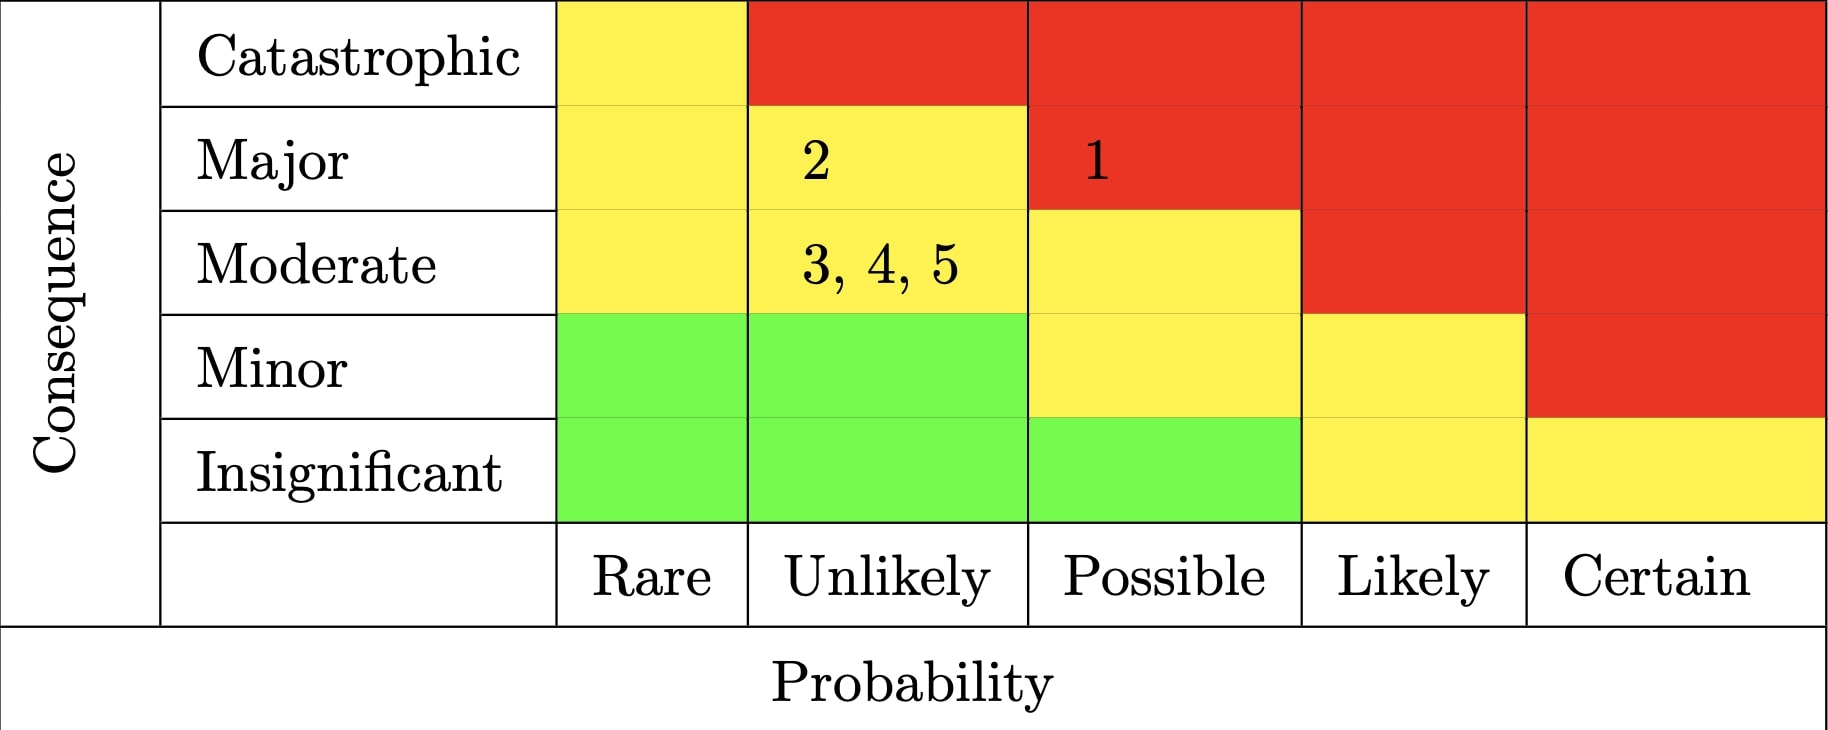
\includegraphics[width=1\columnwidth]{Images/RiskAnalysis1.jpeg}
\begin{table}[!ht] 
    \centering
    \begin{tabular}{|l|l|l|l|l|l|l|l|l|l|}
    \hline
    \multirow{6}{*}{\rotatebox[origin=c]{90}{Consequence}}
        ~ & Catastrophic & \cellcolor{yellow!} & \cellcolor{red} & \cellcolor{red} & \cellcolor{red} & \cellcolor{red}  \\ \cline{2-7}
        ~ & Major & \cellcolor{yellow!} & \cellcolor{yellow!} 2 & \cellcolor{red} 1 & \cellcolor{red} & \cellcolor{red} \\ \cline{2-7}
        ~ & Moderate & \cellcolor{yellow!} & \cellcolor{yellow!} 3, 4, 5 & \cellcolor{yellow!} & \cellcolor{red} & \cellcolor{red} \\ \cline{2-7}
        ~ & Minor & \cellcolor{green!} & \cellcolor{green!} & \cellcolor{yellow!} & \cellcolor{yellow!} & \cellcolor{red} \\ \cline{2-7}
        ~ & Insignificant & \cellcolor{green!} & \cellcolor{green!} & \cellcolor{green!} & \cellcolor{yellow!} & \cellcolor{yellow!} \\ \cline{2-7}
       ~ & ~ & Rare & Unlikely & Possible & Likely & Certain ~ \\ \hline
        \multicolumn{7}{|c|}{Probability}
        \\ \hline
    \end{tabular}
    \caption{Risk matrix \cite{risk-matrix}}
\end{table}

\vspace{1cm}
    \begin{table}[!ht]
    \raggedright
    \textbf{Risk scenario 1:}
    \\
    \centering
    \begin{tabular}{|p{0.2\textwidth}|p{0.8\textwidth}|}
    \hline
        Risk scenario & Stretching beyond scope \\ \hline
        Description & Due to poor planing and communication in the group, the group have taken on too much and this leads to a larger scope. This leads to that the group cannot deliver on the original task \\ \hline   
        Probability & Possible  \\ \hline
        Consequence & Major  \\ \hline   
        Overall risk & \cellcolor{red!} Very serious  \\ \hline
    
    \end{tabular}
    \caption{Scenario 1}
    \raggedright
    \textbf{Measures:}
    \\ 
    By implementing proper oversight and developing a solid project plan will result in  minimizing potential harm. Additionally, before making any decisions to expand the project, it is important to thoroughly assess the necessity of doing so in order to prevent scope creep.
\end{table}


\vspace{1cm}
\begin{table}[!ht]
    \raggedright
    \textbf{Risk scenario 2:}
    \\~
    \centering
    \begin{tabular}{|p{0.2\textwidth}|p{0.8\textwidth}|}
    \hline
        Risk scenario & Loss of data \\ \hline
        Description & The group will lose important data or documents  \\ \hline
        Probability & Unlikely \\ \hline
        Consequence & Major \\ \hline
        Overall risk & \cellcolor{yellow!} Moderate \\ \hline
    \end{tabular}
    \caption{Scenario 2}
    \raggedright
    \textbf{Measures:}
    \\ 
    To mitigate this risk, the group need to ensure that our data is stored in multiple locations and devices. Regular backups should also be performed to these locations to minimize loss in the event of an incident.
\end{table}


\vspace{2cm}
\begin{table}[!ht]
    \raggedright
    \textbf{Risk scenario 3:}
    \\
    \centering
    \begin{tabular}{|p{0.2\textwidth}|p{0.8\textwidth}|}
    \hline
        Risk scenario & Group conflict \\ \hline
        Description & Group will disagree   \\ \hline
        Probability & Unlikely \\ \hline
        Consequence & Moderate \\ \hline
        Overall risk &  \cellcolor{yellow!} Moderate \\ \hline
    \end{tabular}
    \caption{Scenario 3}
    \raggedright
    \textbf{Measures:}
    \\ 
    Encourage open communication among group members and actively listen to each other's perspectives. Identify the root causes of the conflict and work to address them directly. If the conflict cannot be resolved within the group, consider seeking assistance from a neutral counselor.
\end{table}

\vspace{2cm}
\begin{table}[!ht]
    \raggedright
    \textbf{Risk scenario 4:}
    \\
    \centering
    \begin{tabular}{|p{0.2\textwidth}|p{0.8\textwidth}|}
    \hline
        Risk scenario & Loss of contact with stakeholder\\ \hline
        description & For some reason we cannot reach the stakeholder and they do not respond to us  \\ \hline
        Probability & Unlikely  \\ \hline
        Consequence & Moderate  \\ \hline
        Overall risk & \cellcolor{yellow!} Moderate \\ \hline
    \end{tabular}
    \caption{Scenario 4}
    \raggedright
    \textbf{Measures:}
    \\ 
    Initially, the group would attempt to contact individuals through email. If this is unsuccessful, Celina, one of the group members, will contact the stakeholder at work since she works at NBIM. In the worst case the group could finish this task without them since we don't need access to their systems.
\end{table}

\vspace{2cm}
\begin{table}[!ht]
    \raggedright
    \textbf{Risk scenario 5:}
    \\
    \centering
    \begin{tabular}{|p{0.2\textwidth}|p{0.8\textwidth}|}
    \hline
        Risk scenario & A group member gets sick \\ \hline
        Description & Due to a new pandemic or other circumstances, a group member may become ill and unable to contribute to the group's efforts, resulting in the group having to redistribute the workload among fewer members. \\ \hline
        Probability & Unlikely  \\ \hline
        Consequence & Moderate  \\ \hline
        Overall risk & \cellcolor{yellow!} Moderate \\ \hline
    \end{tabular}
    \caption{Scenario 5}
    \raggedright
    \textbf{Measures:}
    \\
    It is difficult prevent someone from becoming sick, however our effective documentation and god communication allow for continuation of work by others in the event that a team member falls ill.
\end{table}

\clearpage
\section{Plan for execution}
\subsection{Gantt chart}
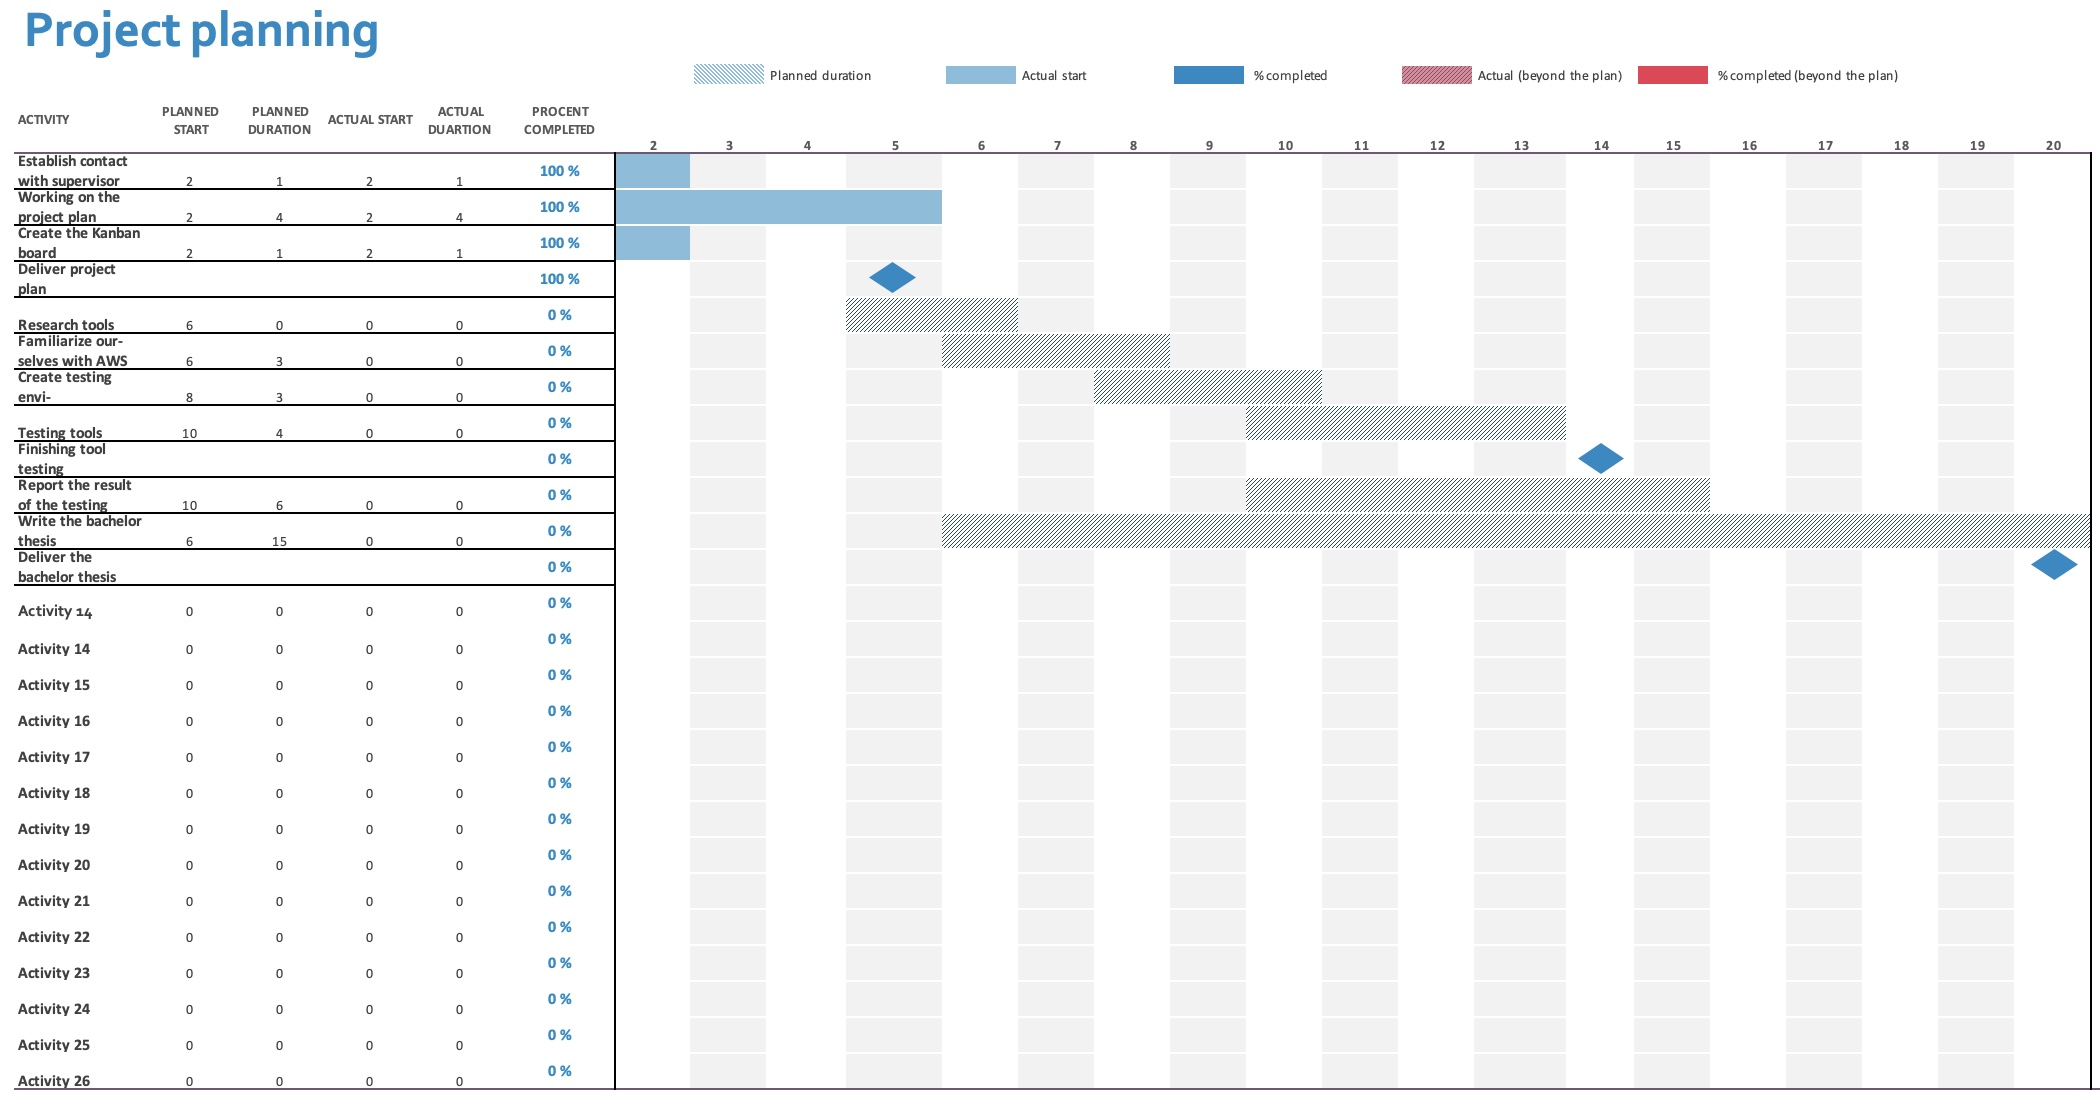
\includegraphics[width=1\columnwidth]{Images/gantt2.jpg}
\\

\newpage

\newpage
\section{Signature}

\begin{tabular}{@{}p{.5in}p{4in}@{}}\\
Approved: & \hrulefill \\
& Anniken Arildset \\
\\
Approved: & \hrulefill \\
& Celina Heimdal Brynildsen \\
\\
Approved: & \hrulefill \\
& Sebastian Hestsveen \\
\\
Approved: & \hrulefill \\
& Thea Urne
\\~\\
\end{tabular}
\newpage








% End of document
\end{document}
